\documentclass[11pt,a4paper]{article}

\usepackage[T1]{fontenc}
\usepackage[margin=1in]{geometry}
\usepackage{microtype}
\usepackage{amsmath,amssymb,amsthm,mathtools}
\usepackage{booktabs,array,tabularx}
\usepackage{enumitem}
\usepackage{xcolor}
\usepackage{tikz}
\usetikzlibrary{arrows.meta,positioning,shapes.geometric,fit,calc,backgrounds}
\usepackage{pgfplots}
\pgfplotsset{compat=1.18}
\usepackage{caption}
\usepackage{placeins}
\usepackage{xurl}
\usepackage{hyperref}
\usepackage[nameinlink,noabbrev]{cleveref}

% Color palette
\definecolor{Navy}{HTML}{1B365D}
\definecolor{Teal}{HTML}{00695C}
\definecolor{Crimson}{HTML}{A61C3C}
\definecolor{Slate}{HTML}{455A64}
\definecolor{LightBlue}{HTML}{EBF2FA}
\definecolor{LightTeal}{HTML}{E6F4F1}
\definecolor{LightRed}{HTML}{FCEEEF}
\definecolor{LightGray}{HTML}{F5F7FA}

\hypersetup{
  colorlinks=true,
  linkcolor=Navy,
  citecolor=Teal,
  urlcolor=Navy,
  pdftitle={Rigorous Resolution of the Two-Qubit Maximal Magic Conjecture via SO(6) Geometry and Certified Equivariant Sum-of-Squares Proofs},
  pdfauthor={LingyeNBird}
}

% Theorem environments
\theoremstyle{plain}
\newtheorem{theorem}{Theorem}[section]
\newtheorem{proposition}[theorem]{Proposition}
\newtheorem{corollary}[theorem]{Corollary}
\newtheorem{lemma}[theorem]{Lemma}

\theoremstyle{definition}
\newtheorem{definition}[theorem]{Definition}
\newtheorem{example}[theorem]{Example}

\theoremstyle{remark}
\newtheorem{remark}[theorem]{Remark}

% Mathematical macros
\newcommand{\C}{\mathbb{C}}
\newcommand{\R}{\mathbb{R}}
\newcommand{\Z}{\mathbb{Z}}
\newcommand{\Q}{\mathbb{Q}}
\newcommand{\N}{\mathbb{N}}
\newcommand{\F}{\mathbb{F}}
\newcommand{\ket}[1]{\lvert #1 \rangle}
\newcommand{\bra}[1]{\langle #1 \rvert}
\newcommand{\braket}[2]{\langle #1 \vert #2 \rangle}
\newcommand{\ketbra}[2]{\lvert #1 \rangle\langle #2 \rvert}
\newcommand{\expval}[2]{\langle #1 \vert #2 \vert #1 \rangle}
\newcommand{\Tr}{\operatorname{Tr}}
\newcommand{\Pf}{\operatorname{Pf}}
\newcommand{\sgn}{\operatorname{sgn}}
\newcommand{\SO}{\mathrm{SO}}
\newcommand{\SU}{\mathrm{SU}}
\newcommand{\PSU}{\mathrm{PSU}}
\newcommand{\PSO}{\mathrm{PSO}}
\newcommand{\Spin}{\mathrm{Spin}}
\newcommand{\Sp}{\mathrm{Sp}}
\newcommand{\Cl}{\mathrm{Cl}}
\newcommand{\PCl}{\overline{\mathrm{Cl}}}
\newcommand{\Pauli}{\mathcal{P}}
\newcommand{\Mman}{\mathcal{M}_6}
\newcommand{\Bplus}{B_6^+}
\newcommand{\PBplus}{PB_6^+}
\newcommand{\psimub}{\ket{\psi_{\mathrm{MUB}}}}
\newcommand{\code}[1]{\texttt{\small #1}}

\title{\bfseries\Large Rigorous Resolution of the Two-Qubit Maximal Magic Conjecture via $\SO(6)$ Geometry and Certified Equivariant Sum-of-Squares Proofs}

\author{
  LingyeNBird\thanks{Independent Researcher. Lean~4 formalization, discovery scripts, and standalone Python verifier are available at \url{https://github.com/LingyeNBird/two-qubit-maximal-magic} (release tag \code{v1.0}).}
}

\date{\today}

\begin{document}

\maketitle

\begin{abstract}
Stabilizer R\'enyi Entropies (SREs) $M_\alpha$ form an operationally faithful family of magic monotones for pure quantum states precisely for $\alpha \ge 2$. While Weyl--Heisenberg symmetric informationally complete (WH-SIC) fiducial states saturate the universal upper bound whenever a Pauli-covariant SIC-POVM exists ($n = 1, 3$ qubits), no such POVM exists for two qubits ($n = 2$, the two-qubit instance of Open Quantum Problem~E28), where Liu, Low, and Yin [\textit{Quantum Sci.\ Technol.}\ \textbf{11}, 015035 (2026)] presented numerical evidence that $\max M_2 = \ln(16/7) < \ln(5/2)$. We give a complete, rigorous proof of this conjecture and all of its structural refinements for every R\'enyi order $\alpha \ge 2$: (i) the sharp upper bound $M_\alpha(\ket{\psi}) \le \frac{1}{1-\alpha}\ln\!\bigl((1+3\cdot 4^{1-\alpha})/4\bigr)$, reducing to $\max M_2 = \ln(16/7)$; (ii) complete classification of all maximizers as a single two-qubit Clifford orbit of exact cardinality $480$, coinciding precisely with the two-qubit Pauli $5$-MUB fiducial states; and (iii) the exact Wootters concurrence dichotomy $C(\ket{\psi}) \in \{1/2, 1/\sqrt{2}\}$ with exactly $192$ states at $C = 1/2$ and $288$ at $C = 1/\sqrt{2}$. Our proof combines an $\SU(4) \cong \Spin(6)$ embedding of pure two-qubit states onto the positively oriented skew-orthogonal manifold $\Mman \subset \SO(6)$---yielding a $K_6$ graph dictionary that explains Pauli commutation, Clifford symmetries, MUB structure, and the $192/288$ concurrence split---with an exact rational degree-$8$ $\Bplus$-equivariant sum-of-squares certificate discovered via zero-set face restriction on the extremizer set and rank-$1$ Frank--Wolfe optimization. The exact algebraic identity is verified both by a standalone zero-dependency Python script and inside Lean~4's pure kernel ($32$ audited declarations using standard foundational axioms only).
\end{abstract}

\tableofcontents
\bigskip

%==============================================================================
\section{Introduction}
\label{sec:intro}
%==============================================================================

Quantum computation achieves advantage over classical simulation only when non-Clifford resources---collectively termed \emph{magic} or \emph{nonstabilizerness}---are injected into stabilizer circuits~\cite{BravyiKitaev2005,Veitch2014}. Quantifying magic in a form that is both operationally faithful and computationally tractable has become a central theme across fault-tolerant quantum computing, quantum many-body physics, and quantum foundations. Among computable measures of magic, the \emph{Stabilizer R\'enyi Entropies} (SREs) introduced by Leone, Oliviero, and Hamma~\cite{LeoneOlivieroHamma2022} stand out because they require no convex-roof or polytope minimization for pure states and are directly measurable via randomized measurements.

For an $n$-qubit pure state $\ket{\psi} \in (\C^2)^{\otimes n}$ of dimension $d = 2^n$, let $\Pauli_n = \{I, X, Y, Z\}^{\otimes n}$ denote the $d^2$ unsigned $n$-qubit Pauli operators. The normalized probabilities $\Xi_P(\ket{\psi}) = d^{-1} \lvert\expval{\psi}{P}\rvert^2$ form a probability distribution over $\Pauli_n$ ($\sum_{P\in\Pauli_n} \Xi_P = 1$ by purity $\Tr(\rho^2)=1$), and the order-$\alpha$ SRE is defined as
\begin{equation}
  \label{eq:sre-def}
  M_\alpha(\ket{\psi})
  \;=\; \frac{1}{1-\alpha} \ln\!\left(\frac{1}{d} \sum_{P \in \Pauli_n} \lvert\expval{\psi}{P}\rvert^{2\alpha}\right)
  \;=\; \frac{1}{1-\alpha} \ln\!\left(\sum_{P \in \Pauli_n} \Xi_P(\ket{\psi})^\alpha\right) - \ln d.
\end{equation}
Although Haug and Piroli~\cite{HaugPiroli2023} demonstrated via explicit counterexamples that $M_\alpha$ fails to be monotonic under stabilizer protocols with computational-basis measurements for $0 \le \alpha < 2$, Leone and Bittel~\cite{LeoneBittel2024} subsequently proved that $M_\alpha$ is a genuine resource monotone for pure states precisely in the regime $\alpha \ge 2$. Characterizing the maximum possible value of $M_\alpha$ and the exact extremal states for $\alpha \ge 2$ is therefore fundamental to the resource theory of magic.

\subsection{The WH-SIC Gap, Liu--Low--Yin's Conjecture, and Problem E28}

Since $\expval{\psi}{I} = 1$ and $\sum_{P \neq I} \lvert\expval{\psi}{P}\rvert^2 = d - 1$ for any pure state, applying Cauchy--Schwarz (or Jensen's inequality for $\alpha > 1$) over the $d^2 - 1$ non-identity Pauli operators immediately gives the universal lower bound
\begin{equation}
  \label{eq:sic-moment-bound}
  \sum_{P \in \Pauli_n} \lvert\expval{\psi}{P}\rvert^{2\alpha}
  \;\ge\; 1 + (d^2 - 1)\left(\frac{d - 1}{d^2 - 1}\right)^{\!\alpha}
  \;=\; 1 + (d^2 - 1)(d + 1)^{-\alpha},
\end{equation}
which translates into the upper bound
\begin{equation}
  \label{eq:sic-sre-bound}
  M_\alpha(\ket{\psi}) \;\le\; M_\alpha^{\mathrm{SIC}}(d)
  \;:=\; \frac{1}{1-\alpha}\ln\!\left(\frac{1 + (d^2-1)(d+1)^{-\alpha}}{d}\right).
\end{equation}
Cuffaro and Fuchs~\cite{CuffaroFuchs2024} observed that equality in~\eqref{eq:sic-sre-bound} holds if and only if $\lvert\expval{\psi}{P}\rvert = 1/\sqrt{d+1}$ for all $d^2 - 1$ non-identity displacement operators, i.e., precisely when $\ket{\psi}$ is a fiducial state of a Weyl--Heisenberg Symmetric Informationally Complete POVM (WH-SIC)~\cite{Zauner1999,Renes2004} covariant under the relevant displacement group.

For a single qubit ($n=1$, $d=2$), the Pauli group $\Pauli_1$ coincides with the cyclic $\Z_2$ Weyl--Heisenberg group and admits a WH-SIC (the tetrahedron states), so $M_2^{\max}(n=1) = \ln(3/2) = M_2^{\mathrm{SIC}}(2)$ is attained. Likewise, in $n=3$ ($d=8$), Hoggar lines~\cite{Hoggar1998} provide a $\Pauli_3$-covariant SIC-POVM saturating~\eqref{eq:sic-sre-bound}. However, Godsil and Roy~\cite{GodsilRoy2009} proved that a $\Pauli_n$-covariant SIC-POVM exists \emph{only} for $n=1$ and $n=3$. For \textbf{two qubits} ($n=2$, $d=4$), while a WH-SIC exists for the \emph{cyclic} $\Z_4$ clock--shift group in $\C^4$, \textbf{no SIC-POVM covariant under the two-qubit Pauli group $\Pauli_2$ exists}. Consequently, the bound~\eqref{eq:sic-sre-bound} at $d=4$, namely
\begin{equation}
  M_2^{\mathrm{SIC}}(4) \;=\; \ln\!\left(\frac{5}{2}\right) \;\approx\; 0.91629,
\end{equation}
is not attainable.

In a numerical and structural study, Liu, Low, and Yin~\cite{LiuLowYin2026} found strong numerical evidence that for two qubits, the true maximum of $M_2$ is strictly smaller than $\ln(5/2)$, namely
\begin{equation}
  \max_{\substack{\ket{\psi}\in\C^4 \\ \lVert\ket{\psi}\rVert = 1}} M_2(\ket{\psi}) \;=\; \ln\!\left(\frac{16}{7}\right) \;\approx\; 0.82668,
\end{equation}
representing a strict gap of $\ln(35/32) \approx 0.08961$ nats ($\approx 9.78\%$) below the WH-SIC bound (see \Cref{fig:sre-bounds}). They further identified $480$ states saturating $\ln(16/7)$ as Weyl--Heisenberg mutually unbiased basis (MUB) fiducial states generated by the Clifford group---represented up to Clifford equivalence by $\psimub = \tfrac{1}{2}(1, 1, 1, i)^T$---and observed that their Wootters concurrence~\cite{Wootters1998} takes only the two values $1/2$ and $1/\sqrt{2}$ (depending on whether the fifth stabilizer basis completing the MUB set is maximally entangled or separable), so \emph{no} maximal-magic state in this family is maximally entangled. Subsequently, Roman et al.~\cite{Roman2026} mapped the two-qubit magic--entanglement Pareto frontiers for $M_2$ versus concurrence, deriving explicit analytical state families along the boundary that reproduce $\ln(16/7)$ and the $480$ states without proving global exhaustiveness of the upper boundary. Establishing a rigorous analytical proof of $\max M_2 = \ln(16/7)$---and proving that the $480$ MUB fiducial states exhaust all global maximizers (thereby also confirming the global optimality of the peak value and peak-state set on the upper Pareto frontier of~\cite{Roman2026})---was highlighted as a concrete open subproblem in Open Quantum Problem~E28~\cite{OpenQuantumE28} (\emph{``Maximal stabilizer R\'enyi entropy without a Weyl--Heisenberg SIC''}).

\subsection{Main Results}

In this work, we provide a complete, rigorous resolution---combining Lie-theoretic analysis with a machine-verified exact algebraic certificate---of the two-qubit maximal magic conjecture across the entire monotonicity regime $\alpha \ge 2$, establishing for the first time both the global sharp bound and the exhaustiveness of the $480$-state Clifford orbit, together with a purely combinatorial explanation of its MUB and entanglement structure.

\begin{theorem}[Complete Resolution of the Two-Qubit Maximal Magic Conjecture]
\label{thm:main}
Let $\ket{\psi} \in \C^4$ be any normalized pure two-qubit state ($\sum_{i=0}^3 \lvert\psi_i\rvert^2 = 1$), and let $\alpha \ge 2$ be any real R\'enyi order.
\begin{enumerate}[label=\textup{(\roman*)}, leftmargin=2.2em]
  \item \textbf{Sharp upper bound:} The Pauli $2\alpha$-moment and Stabilizer R\'enyi Entropy satisfy
  \begin{equation}
    \label{eq:main-bound}
    \sum_{P \in \Pauli_2} \lvert\expval{\psi}{P}\rvert^{2\alpha} \;\ge\; 1 + 3 \cdot 4^{1-\alpha},
    \qquad
    M_\alpha(\ket{\psi}) \;\le\; \frac{1}{1-\alpha}\ln\!\left(\frac{1 + 3 \cdot 4^{1-\alpha}}{4}\right).
  \end{equation}
  In particular, for $\alpha = 2$,
  \begin{equation}
    \label{eq:main-alpha2}
    \sum_{P \in \Pauli_2} \lvert\expval{\psi}{P}\rvert^{4} \;\ge\; \frac{7}{4},
    \qquad
    M_2(\ket{\psi}) \;\le\; \ln\!\left(\frac{16}{7}\right).
  \end{equation}
  \item \textbf{Exact attainment:} The state $\psimub = \frac{1}{2}(1, 1, 1, i)^T$ attains equality in~\eqref{eq:main-bound} simultaneously for every $\alpha \ge 2$.
  \item \textbf{Pauli spectrum and maximal commuting triple:} Equality holds in~\eqref{eq:main-bound} for some (equivalently, all) $\alpha \ge 2$ if and only if $\lvert\expval{\psi}{P}\rvert \in \{0, \frac{1}{2}\}$ for every $P \in \Pauli_2 \setminus \{I\}$. In this case, exactly $3$ non-identity Pauli expectations vanish---forming a maximal pairwise-commuting Pauli triple---and the remaining $12$ have magnitude $\frac{1}{2}$.
  \item \textbf{Single Clifford orbit and exact cardinality $480$:} Equality holds in~\eqref{eq:main-bound} if and only if $\ket{\psi} = \theta U \psimub$ for some unit global phase $\lvert\theta\rvert = 1$ and some two-qubit Clifford unitary $U \in \Cl_2$. The set of maximizer pure-state density matrices $\{\ketbra{\psi}{\psi}\}$ is finite of exact cardinality $480$.
  \item \textbf{$5$-MUB fiducial equivalence:} Equality holds in~\eqref{eq:main-bound} if and only if $\ket{\psi}$ is a two-qubit Pauli (multi-qubit Weyl--Heisenberg) $5$-MUB fiducial state, meaning that its $16$-state Pauli orbit $\{P\ket{\psi} : P \in \Pauli_2\}$ partitions into $4$ orthonormal bases extending to a complete set of $d+1 = 5$ mutually unbiased bases in $\C^4$.
  \item \textbf{Entanglement dichotomy and exact $192/288$ distribution:} Every maximizer $\ket{\psi}$ has Wootters concurrence
  \begin{equation}
    C(\ket{\psi}) \;=\; 2\lvert\psi_0\psi_3 - \psi_1\psi_2\rvert \;=\; \sqrt{2\bigl(1 - \Tr(\rho_A^2)\bigr)} \;\in\; \left\{\frac{1}{2},\; \frac{1}{\sqrt{2}}\right\},
  \end{equation}
  so $0 < C(\ket{\psi}) < 1$ strictly (no maximizer is separable or maximally entangled). Among the $480$ maximizer density matrices, exactly $192$ satisfy $C = \frac{1}{2}$ and exactly $288$ (including $\psimub$) satisfy $C = \frac{1}{\sqrt{2}}$.
\end{enumerate}
\end{theorem}

\begin{remark}[Scope and conventions]
Throughout this paper we use the natural logarithm $\ln$ in~\eqref{eq:sre-def}; dividing by $\ln 2$ gives the base-$2$ value $\log_2(16/7) \approx 1.19265$ bits, while the core moment inequality in~\eqref{eq:main-bound} is base-independent. We emphasize two explicit scope boundaries: first, while $n=1$ (tetrahedron states) and $n=3$ (Hoggar lines) saturate the WH-SIC bound $M_\alpha^{\mathrm{SIC}}(2^n)$~\cite{CuffaroFuchs2024} and \Cref{thm:main} resolves the two-qubit ($n=2$) case of Open Quantum Problem~E28 across all $\alpha \ge 2$, higher non-SIC multi-qubit systems ($n \ge 4$, including Liu--Low--Yin's general $n$-qubit conjecture for $n \neq 1, 3$~\cite{LiuLowYin2026}) remain open; second, following multi-qubit quantum information convention, the displacement group in (v) is the two-qubit Pauli group $\Pauli_2 = \{I, X, Y, Z\}^{\otimes 2}$ rather than the cyclic $\Z_4$ clock--shift group.
\end{remark}

\begin{figure}[tbp]
  \centering
  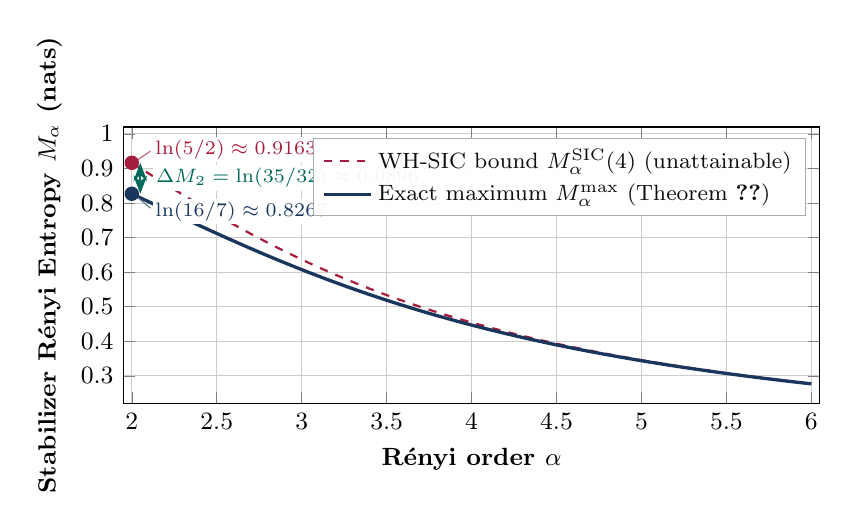
\begin{tikzpicture}
    \begin{axis}[
      width=0.86\textwidth,
      height=0.42\textwidth,
      xlabel={R\'enyi order $\alpha$},
      ylabel={Stabilizer R\'enyi Entropy $M_\alpha$ (nats)},
      xmin=1.95, xmax=6.05,
      ymin=0.22, ymax=1.02,
      xtick={2,2.5,3,3.5,4,4.5,5,5.5,6},
      ytick={0.3,0.4,0.5,0.6,0.7,0.8,0.9,1.0},
      grid=both,
      grid style={line width=.2pt, draw=gray!25},
      major grid style={line width=.35pt, draw=gray!40},
      legend style={
        at={(0.98,0.96)},
        anchor=north east,
        font=\footnotesize,
        draw=Slate!50,
        fill=white,
        fill opacity=0.95,
        cells={anchor=west}
      },
      tick label style={font=\small},
      label style={font=\small\bfseries}
    ]
      % WH-SIC upper bound (d=4)
      \addplot[
        color=Crimson,
        thick,
        dashed,
        domain=2:6,
        samples=120
      ] {(1/(1-x))*ln((1 + 15*(5^(-x)))/4)};
      \addlegendentry{WH-SIC bound $M_\alpha^{\mathrm{SIC}}(4)$ (unattainable)}

      % Exact sharp bound proved in Theorem 1.1
      \addplot[
        color=Navy,
        very thick,
        domain=2:6,
        samples=120
      ] {(1/(1-x))*ln((1 + 3*(4^(1-x)))/4)};
      \addlegendentry{Exact maximum $M_\alpha^{\max}$ (Theorem~\ref{thm:main})}

      % Highlight alpha = 2 points and gap
      \addplot[only marks, mark=*, mark size=2.4pt, color=Crimson] coordinates {(2, 0.916291)};
      \addplot[only marks, mark=*, mark size=2.4pt, color=Navy] coordinates {(2, 0.826679)};

      % Vertical double arrow for gap at alpha = 2
      \draw[<->, >=Stealth, thick, Teal] (axis cs:2.05, 0.826679) -- (axis cs:2.05, 0.916291);
      \node[anchor=west, font=\scriptsize, text=Teal, fill=white, inner sep=1.2pt]
        at (axis cs:2.12, 0.872) {$\Delta M_2 = \ln(35/32) \approx 0.0896$};

      \node[anchor=west, font=\scriptsize, text=Crimson, fill=white, inner sep=1pt]
        at (axis cs:2.12, 0.955) {$\ln(5/2) \approx 0.9163$};
      \node[anchor=west, font=\scriptsize, text=Navy, fill=white, inner sep=1pt]
        at (axis cs:2.12, 0.775) {$\ln(16/7) \approx 0.8267$};
      \draw[Navy!70, thin] (axis cs:2.02, 0.822) -- (axis cs:2.11, 0.785);
      \draw[Crimson!70, thin] (axis cs:2.02, 0.920) -- (axis cs:2.11, 0.950);
    \end{axis}
  \end{tikzpicture}
  \caption{Comparison between the naive Weyl--Heisenberg SIC upper bound $M_\alpha^{\mathrm{SIC}}(4) = \frac{1}{1-\alpha}\ln\bigl((1 + 15\cdot 5^{-\alpha})/4\bigr)$ (dashed red) and the exact sharp two-qubit maximum $M_\alpha^{\max} = \frac{1}{1-\alpha}\ln\bigl((1 + 3\cdot 4^{1-\alpha})/4\bigr)$ proved in \Cref{thm:main} (solid navy) across the entire monotonicity regime $\alpha \ge 2$~\cite{LeoneBittel2024}. At $\alpha = 2$, the exact bound improves on $M_2^{\mathrm{SIC}}(4)$ by $\ln(35/32) \approx 0.0896$ nats ($\approx 9.78\%$).}
  \label{fig:sre-bounds}
\end{figure}

\subsection{Conceptual and Methodological Contributions}

Beyond resolving the conjecture, this paper combines two complementary ingredients:

\paragraph{1. The $\SO(6)/K_6$ Geometric Dictionary.}
The naive sphere bound~\eqref{eq:sic-moment-bound} ignores the nonlinear algebraic constraints satisfied by pure two-qubit Pauli expectations. Via the exceptional isomorphism $\SU(4) \cong \Spin(6)$ ($\mathfrak{su}(4) \cong \mathfrak{so}(6) \cong \Lambda^2 \R^6$)~\cite{FultonHarris1991}, the $15$ signed Pauli expectations of a pure two-qubit state assemble into a real $6\times 6$ skew-symmetric orthogonal matrix $A \in \SO(6)$ satisfying $A^2 = -I_6$ and the orientation (Pfaffian) condition $\Pf(A) = +1$. This recasts the two-qubit Pauli algebra onto the complete graph $K_6$: Pauli commutation becomes edge disjointness, maximal commuting triples become perfect matchings, every signed permutation in the rotational hyperoctahedral group $\Bplus$ (acting via the order-$11{,}520$ quotient $\PBplus = \Bplus/\{\pm I_6\} \cong \PCl_2$) is realized by a two-qubit Clifford unitary, and the local qubit-$A$ and qubit-$B$ Bloch vectors become two complementary triangles $T_A, T_B \subset K_6$. Once the extremal Pauli spectrum forces the vanishing edges to form a perfect matching $M$ of $K_6$, the $192/288$ concurrence dichotomy follows in three lines: a matching of $K_6$ can intersect a triangle $T_A$ in either $0$ edges ($6$ bipartite matchings $\implies C = 1/2$) or $1$ edge ($9$ matchings $\implies C = 1/\sqrt{2}$).

\paragraph{2. Exact Equivariant Sum-of-Squares Certification via Witnessed Orbit Cancellation.}
Proving the sharp quartic inequality $\min_{A\in\Mman}\sum_e a_e^4 = 3/4$ requires certifying a non-convex polynomial bound whose minimum is attained on a $480$-point extremizer set. Because every valid SOS Gram matrix must vanish on the extremizers, it is necessarily \emph{rank-deficient} (singular), ruling out floating-point perturbation/padding certification tools (such as \textsc{ValidSDP}~\cite{MartinDorelRoux2017,Roux2018}) that require strict positive definiteness. Following established techniques in facial reduction~\cite{PermenterParrilo2018}, symmetric SOS optimization~\cite{GatermannParrilo2004,Riener2013}, and exact rational SOS certification~\cite{PeyrlParrilo2008,Kaltofen2008,Kaltofen2012,MagronSafeyElDin2018}, we construct an exact rational degree-$8$ $\Bplus$-equivariant SOS certificate by: (a) restricting to a $46$-dimensional integer basis of the PSD-cone face determined by the $480$ extremizers while pinning $Q_1(a) = 4a_0^3 - a_0$; (b) solving a low-rank primal-dual Frank--Wolfe SDP to obtain $7$ sparse integer squares, followed by exact $\Q$-linear solves for positive weights and local ideal cofactors; and (c) encoding the vanishing of the $\Bplus$-symmetrized remainder $F$ ($1{,}409$ monomials) via per-monomial orbit-cancellation witnesses (\Cref{lem:orbit-cancel}). While an external script exploiting the diagonal sign subgroup $(\Z/2\Z)^5 \subset \Bplus$ can check the $S_6$-reduced average ($720 \times 1{,}409 \approx 1.01\times 10^6$ actions) directly in under a second, encoding the Reynolds-operator cancellation as $1{,}409$ explicit $\Bplus$ witnesses reduces the verification work to $O(\lvert F\rvert \log \lvert F\rvert)$---an order-of-magnitude reduction ($\sim 70\times$) even relative to parity-reduced $S_6$ averaging, and three orders of magnitude relative to generic $\lvert\Bplus\rvert$-averaging---making pure-kernel (\code{rfl}) machine verification practical inside Lean~4~\cite{deMouraUllrich2021,Mathlib2020} without formalizing group-specific semidirect-product decompositions. Both a standalone Python verifier (\code{scripts/verify\_certificate.py}) and the complete Lean~4 formalization ($32$ audited declarations) are publicly provided.

\paragraph{Paper organization.}
\Cref{sec:so6} constructs the $\SO(6)$ embedding and the $K_6$ geometric dictionary. \Cref{sec:sos-bound} establishes the exact $\alpha = 2$ SOS identity, extracts the extremal Pauli spectrum, and lifts the bound to all $\alpha \ge 2$ via H\"older's inequality. \Cref{sec:maximizers} proves the single Clifford orbit theorem, exact cardinality $480$, and $5$-MUB fiducial equivalence. \Cref{sec:entanglement} proves the concurrence dichotomy and exact $192/288$ split via $K_6$ triangle intersections. \Cref{sec:methodology} documents the reproducible certificate-discovery pipeline and witnessed orbit cancellation. \Cref{sec:discussion} discusses open problems ($n \ge 4$ qubits, $0 < \alpha < 2$, and bipartite qudits) and computational bottlenecks. \Cref{app:explicit} lists the explicit $4\times 4$ Clifford generators and standalone certificate files, and \Cref{app:lean} summarizes the Lean~4 pure-kernel implementation and audited theorem index.

\FloatBarrier
%==============================================================================
\section{The \texorpdfstring{$\SO(6)$}{SO(6)} Geometry of Two-Qubit Pure States and the \texorpdfstring{$K_6$}{K6} Dictionary}
\label{sec:so6}
%==============================================================================

Let $\ket{\psi} = (\psi_0, \psi_1, \psi_2, \psi_3)^T \in \C^4$ satisfy $\sum_{j=0}^3 \lvert\psi_j\rvert^2 = 1$, where the computational basis is ordered as $\ket{00}, \ket{01}, \ket{10}, \ket{11}$. We index the single-qubit Pauli matrices as $\sigma_0 = I$, $\sigma_1 = X$, $\sigma_2 = Y$, $\sigma_3 = Z$, and write $P_{a,b} = \sigma_a \otimes \sigma_b \in \Pauli_2$ for $a, b \in \{0,1,2,3\}$. Each $P_{a,b}$ is Hermitian and unitary, so $\expval{\psi}{P_{a,b}} \in \R$.

\subsection{The Skew-Orthogonal Manifold \texorpdfstring{$\Mman \subset \SO(6)$}{M6 subset SO(6)}}

Under the exceptional Lie group isomorphism $\SU(4) \cong \Spin(6)$~\cite{FultonHarris1991}, the $15$-dimensional real vector space $i\,\mathfrak{su}(4)$ of traceless $4\times 4$ Hermitian matrices is canonically isomorphic (as an $\SU(4)$-representation) to $\mathfrak{so}(6) \cong \Lambda^2 \R^6$, the space of $6\times 6$ real skew-symmetric matrices. Concretely, label the $15$ ordered edges of the complete graph $K_6$ on vertex set $V(K_6) = \{0,1,2,3,4,5\}$ in lexicographic order $e = 0, \dots, 14$ as $(i_e, j_e)$ with $i_e < j_e$, and assign to each edge $e$ a signed non-identity Pauli operator $\tilde{P}_e = s_e P_{a_e, b_e}$ ($s_e \in \{\pm 1\}$) according to \Cref{tab:k6-dict}.

\begin{table}[htbp]
  \centering
  \caption{The explicit $K_6$ Pauli dictionary $\tilde{P}_e = s_e P_{a_e, b_e}$ realizing $\mathfrak{su}(4) \cong \mathfrak{so}(6)$ via $-\frac{i}{2}\tilde{P}_e \mapsto E_{i_e j_e} - E_{j_e i_e}$. Local qubit-$A$ Paulis form the triangle $T_A = \{0,1,5\}$ (edges $0,4,8$); local qubit-$B$ Paulis form the complementary triangle $T_B = \{2,3,4\}$ (edges $9,10,12$). The column $a_e(\psimub) = \expval{\psi_{\mathrm{MUB}}}{\tilde{P}_e}$ records the values for $\psimub = \frac{1}{2}(1,1,1,i)^T$, whose three zeros $\{0, 9, 14\} \leftrightarrow \{ZI, IZ, ZZ\}$ form a perfect matching of $K_6$.}
  \label{tab:k6-dict}
  \footnotesize
  \setlength{\tabcolsep}{4.5pt}
  \begin{tabular}{@{}cccrc@{\qquad}cccrc@{}}
    \toprule
    Edge $e$ & $(i_e, j_e)$ & $\tilde{P}_e$ & $a_e(\psimub)$ & Sector &
    Edge $e$ & $(i_e, j_e)$ & $\tilde{P}_e$ & $a_e(\psimub)$ & Sector \\
    \midrule
    $0$  & $(0,1)$ & $+ZI$ & $0$     & $T_A$ (loc.\ $A$) &
    $8$  & $(1,5)$ & $-YI$ & $-1/2$  & $T_A$ (loc.\ $A$) \\
    $1$  & $(0,2)$ & $-YX$ & $-1/2$  & $T_A \leftrightarrow T_B$ &
    $9$  & $(2,3)$ & $+IZ$ & $0$     & $T_B$ (loc.\ $B$) \\
    $2$  & $(0,3)$ & $+YY$ & $+1/2$  & $T_A \leftrightarrow T_B$ &
    $10$ & $(2,4)$ & $-IY$ & $-1/2$  & $T_B$ (loc.\ $B$) \\
    $3$  & $(0,4)$ & $+YZ$ & $-1/2$  & $T_A \leftrightarrow T_B$ &
    $11$ & $(2,5)$ & $-ZX$ & $-1/2$  & $T_A \leftrightarrow T_B$ \\
    $4$  & $(0,5)$ & $+XI$ & $+1/2$  & $T_A$ (loc.\ $A$) &
    $12$ & $(3,4)$ & $-IX$ & $-1/2$  & $T_B$ (loc.\ $B$) \\
    $5$  & $(1,2)$ & $-XX$ & $-1/2$  & $T_A \leftrightarrow T_B$ &
    $13$ & $(3,5)$ & $+ZY$ & $-1/2$  & $T_A \leftrightarrow T_B$ \\
    $6$  & $(1,3)$ & $+XY$ & $+1/2$  & $T_A \leftrightarrow T_B$ &
    $14$ & $(4,5)$ & $+ZZ$ & $0$     & $T_A \leftrightarrow T_B$ \\
    $7$  & $(1,4)$ & $+XZ$ & $+1/2$  & $T_A \leftrightarrow T_B$ &
         &         &       &         & \\
    \bottomrule
  \end{tabular}
\end{table}

Given any $a = (a_0, \dots, a_{14}) \in \R^{15}$, let $A = \mathrm{Skew}(a) \in \R^{6\times 6}$ denote the unique skew-symmetric matrix with $A_{i_e, j_e} = a_e = -A_{j_e, i_e}$ and $A_{ii} = 0$. Define the $\SO(6)$-equivariant quadratic Pfaffian (orientation) operator $\Phi(A) \in \R^{6\times 6}$ by
\begin{equation}
  \label{eq:hodge-phi}
  \Phi(A)_{ij} \;:=\; \sum_{\substack{\sigma \in S_6 \\ \sigma(0) = i,\; \sigma(1) = j}} \sgn(\sigma)\, A_{\sigma(2)\sigma(3)}\, A_{\sigma(4)\sigma(5)}.
\end{equation}
For $(i,j) = (0,1)$, the $4! = 24$ permutations fixing $0$ and $1$ partition into $3$ matchings of $\{2,3,4,5\}$ with $8$-fold multiplicity each, giving
\begin{equation}
  \label{eq:hodge-01}
  \Phi(A)_{01} \;=\; 8\,(a_9 a_{14} - a_{10} a_{13} + a_{11} a_{12})
  \;=\; 8\,\Pf(A_{\{2,3,4,5\}}).
\end{equation}
More generally, denoting the standard orthonormal basis of $\R^6$ by $\mathbf{e}_0, \dots, \mathbf{e}_5$ and identifying $A \in \mathfrak{so}(6)$ with the $2$-form $\omega_A = \sum_{i<j} A_{ij}\, \mathbf{e}_i \wedge \mathbf{e}_j \in \Lambda^2\R^6$, the operator $\Phi(A)$ encodes $8\,*(\omega_A^{\wedge 2}/2)$, i.e., $8$ times the Hodge dual of the $4$-form $\omega_A^{\wedge 2}/2 \in \Lambda^4\R^6$. When $A^2 = -I_6$, one has $\Pf(A) \in \{\pm 1\}$, and the orientation condition $\Phi(A) = 8A$ (equivalently, $*(\omega_A^{\wedge 2}/2) = \omega_A$) holds if and only if $\Pf(A) = +1$: indeed, if $\Phi(A) = 8A$ then $8\,\Pf(A) = \sum_{j} A_{0j}\Phi(A)_{0j} = 8\sum_j A_{0j}^2 = 8$, giving $\Pf(A) = +1$; conversely, by the real orthogonal normal form of skew-symmetric orthogonal matrices, there exists $R \in \mathrm{O}(6)$ with $A = R J_0 R^T$, where $J_0 = (E_{01}-E_{10}) + (E_{23}-E_{32}) + (E_{45}-E_{54})$ ($E_{ij}$ denoting standard matrix units) satisfies $\Pf(J_0) = +1$ and $\Phi(J_0) = 8J_0$, so $\Pf(A) = \det(R)\Pf(J_0) = +1$ forces $R \in \SO(6)$ and $\SO(6)$-equivariance of $\Phi$ yields $\Phi(A) = R\Phi(J_0)R^T = 8A$.

\begin{definition}[Positively Oriented Skew-Orthogonal Manifold]
\label{def:m6}
We define the real algebraic variety
\begin{equation}
  \label{eq:m6-def}
  \Mman \;:=\; \bigl\{\, a \in \R^{15} \;:\; A = \mathrm{Skew}(a) \text{ satisfies } A^2 = -I_6 \text{ and } \Phi(A) = 8A \,\bigr\}.
\end{equation}
For any pure state $\ket{\psi} \in \C^4$, let $a(\psi) \in \R^{15}$ be defined by $a_e(\psi) := \expval{\psi}{\tilde{P}_e}$ ($e = 0,\dots,14$).
\end{definition}

Geometrically, $\Mman \cong \SO(6)/\mathrm{U}(3) \cong \C\mathbb{P}^3$ is the $6$-dimensional manifold of positively oriented orthogonal complex structures on $\R^6$. Its defining equations immediately encode pure two-qubit states:

\begin{proposition}[$\SO(6)$ Embedding of Pure Two-Qubit States]
\label{prop:so6-embed}
For every normalized pure state $\ket{\psi} \in \C^4$:
\begin{enumerate}[label=\textup{(\alph*)}, leftmargin=2em]
  \item $a(\psi) \in \Mman$, i.e., $A(\psi)^2 = -I_6$ and $\Phi(A(\psi)) = 8A(\psi)$.
  \item In particular, $\sum_{e=0}^{14} a_e(\psi)^2 = 3$, and for every $\alpha > 0$,
  \begin{equation}
    \sum_{P \in \Pauli_2} \lvert\expval{\psi}{P}\rvert^{2\alpha} \;=\; 1 + \sum_{e=0}^{14} \lvert a_e(\psi)\rvert^{2\alpha}.
  \end{equation}
  \item \emph{(Pauli tomography)} Two normalized pure states $\ket{\psi}, \ket{\phi} \in \C^4$ satisfy $a(\psi) = a(\phi)$ if and only if $\ketbra{\psi}{\psi} = \ketbra{\phi}{\phi}$, if and only if $\ket{\phi} = \theta\ket{\psi}$ for some unit global phase $\lvert\theta\rvert = 1$.
\end{enumerate}
\end{proposition}

\begin{proof}
For~(a), direct verification of the commutators across \Cref{tab:k6-dict} confirms that $\iota : \mathfrak{su}(4) \xrightarrow{\sim} \mathfrak{so}(6)$ defined by $\iota\!\left(-\frac{i}{2}\tilde{P}_e\right) = E_{i_e j_e} - E_{j_e i_e}$ is a Lie algebra isomorphism. Since $\SU(4)$ is simply connected, $\iota$ integrates to the double cover $\rho : \SU(4) \to \SO(6)$ intertwining adjoint actions, $\iota(U X U^\dagger) = \rho(U)\,\iota(X)\,\rho(U)^T$. Using the Pauli expansion $\ketbra{\psi}{\psi} = \frac{1}{4}\bigl(I_4 + \sum_{e=0}^{14} a_e(\psi)\tilde{P}_e\bigr)$ (established in~(c) below), we have $A(\psi) = \iota\bigl(-2i(\ketbra{\psi}{\psi} - \frac{1}{4}I_4)\bigr)$, so $A(U\ket{\psi}) = \rho(U)\,A(\psi)\,\rho(U)^T$ for every $U \in \SU(4)$. Because $\SU(4)$ acts transitively on unit vectors in $\C^4$ and both $A^2 = -I_6$ and $\Phi(A) = 8A$ are $\SO(6)$-equivariant, it suffices to check a single reference state $\ket{00}$. On $\ket{00}$, only $a_0 = \expval{00}{ZI} = 1$, $a_9 = \expval{00}{IZ} = 1$, and $a_{14} = \expval{00}{ZZ} = 1$ are nonzero, yielding $A(\ket{00}) = J_0$, which manifestly satisfies $J_0^2 = -I_6$ and $\Phi(J_0) = 8J_0$. (Equivalently, both relations hold directly as polynomial identities in the $8$ real coordinates $(\operatorname{Re}\psi_k, \operatorname{Im}\psi_k)$ modulo $(\sum_{k=0}^3 \lvert\psi_k\rvert^2)^2 = 1$, which is how~(a) is verified directly in \code{SO6Reduction.lean}.) Taking the trace of $A^2 = -I_6$ gives $-2\sum_{e=0}^{14} a_e^2 = \Tr(A^2) = -6$, proving $\sum_e a_e^2 = 3$, while $\expval{\psi}{I} = 1$ and $\lvert a_e(\psi)\rvert = \lvert\expval{\psi}{P_{a_e,b_e}}\rvert$ yield~(b). For~(c), the Hilbert--Schmidt orthogonality $\Tr(P_{a,b} P_{c,d}) = 4\,\delta_{ac}\delta_{bd}$ gives the exact tomographic reconstruction $\ketbra{\psi}{\psi} = \frac{1}{4}\bigl(I + \sum_{e=0}^{14} a_e(\psi)\tilde{P}_e\bigr)$, so $a(\psi) = a(\phi) \iff \ketbra{\psi}{\psi} = \ketbra{\phi}{\phi}$; the equivalence with $\ket{\phi} = \theta\ket{\psi}$ follows by taking $\theta = \phi_k/\psi_k$ for any index $k$ with $\psi_k \neq 0$.
\end{proof}

\subsection{The \texorpdfstring{$K_6$}{K6} Graph Dictionary and Clifford Symmetry}

The assignment in \Cref{tab:k6-dict} is not an arbitrary bijection: it realizes the symplectic geometry of $\Pauli_2$ (whose commutation graph is the complement of the line graph of $K_6$, reflecting $\Sp(4,\F_2) \cong S_6$) directly on $K_6$.

\begin{proposition}[Pauli Commutation $\iff$ $K_6$ Edge Disjointness]
\label{prop:comm-disjoint}
For any two distinct edges $e \neq e'$ of $K_6$ with vertex pairs $(i_e, j_e)$ and $(i_{e'}, j_{e'})$:
\begin{enumerate}[label=\textup{(\alph*)}, leftmargin=2em]
  \item $P_{a_e, b_e}$ and $P_{a_{e'}, b_{e'}}$ commute if and only if $\{i_e, j_e\} \cap \{i_{e'}, j_{e'}\} = \emptyset$;
  \item $P_{a_e, b_e}$ and $P_{a_{e'}, b_{e'}}$ anticommute if and only if $\{i_e, j_e\} \cap \{i_{e'}, j_{e'}\} \neq \emptyset$.
\end{enumerate}
Consequently, a set of non-identity two-qubit Pauli operators is a \emph{maximal pairwise-commuting set} if and only if its corresponding edges form a \emph{perfect matching} of $K_6$ (consisting of $3$ pairwise vertex-disjoint edges). There are exactly $5!! = 15$ such triples.
\end{proposition}

\begin{proof}
Each pair of distinct non-identity Paulis in $\Pauli_2$ either commutes or anticommutes, and direct verification across the $\binom{15}{2} = 105$ pairs in \Cref{tab:k6-dict} confirms that $[P_{a_e, b_e}, P_{a_{e'}, b_{e'}}] = 0$ precisely when $(i_e, j_e)$ and $(i_{e'}, j_{e'})$ share no vertex (equivalently, identifying each edge $\{i,j\}$ of $K_6$ with the weight-$2$ vector $\mathbf{e}_i + \mathbf{e}_j$ in the $4$-dimensional symplectic space $(\F_2^6)_{\mathrm{even}}/\langle\mathbf{1}\rangle$ gives a symplectic isomorphism $(\F_2^6)_{\mathrm{even}}/\langle\mathbf{1}\rangle \xrightarrow{\sim} \F_2^4$ mapping the $15$ edges onto $\F_2^4\setminus\{0\}$). Therefore a pairwise-commuting set of non-identity Paulis corresponds to a matching in $K_6$. Because $K_6$ is a \emph{complete} graph on $6$ vertices, any matching leaving two or more vertices unmatched can be strictly extended by adding the edge between them; hence a matching is maximal if and only if it covers all $6$ vertices (size $3$).
\end{proof}

\begin{remark}[$1$-Factorizations of $K_6$, Complete MUBs, and the Outer Automorphism of $S_6$]
In this dictionary, a partition of the $15$ edges of $K_6$ into $5$ edge-disjoint perfect matchings---a $1$-factorization of $K_6$---corresponds to a partition of $\Pauli_2 \setminus \{I\}$ into $5$ maximal pairwise-commuting triples, whose joint eigenbases form a complete set of $5$ mutually unbiased bases in $\C^4$~\cite{LawrenceBruknerZeilinger2002,KlappeneckerRotteler2004}. There are exactly $6$ such $1$-factorizations (equivalently, $6$ complete stabilizer MUB sets in two qubits); the duality between the $6$ vertices of $K_6$ and its $6$ $1$-factorizations realizes the exceptional outer automorphism of $S_6 \cong \Sp(4,\F_2)$.
\end{remark}

Next, consider the finite \emph{rotational hyperoctahedral group} of $6\times 6$ determinant-$+1$ signed permutation matrices:
\begin{equation}
  \Bplus \;:=\; \bigl\{\, g = (\pi, s) \in S_6 \times \{\pm 1\}^6 \;:\; \sgn(\pi)\prod_{i=0}^5 s_i = +1 \,\bigr\} \;\subset\; \SO(6),
\end{equation}
which has order $\lvert \Bplus\rvert = 6! \cdot 2^5 = 23{,}040$. We realize each $g = (\pi, s) \in \Bplus$ explicitly as the $6\times 6$ orthogonal matrix $g_{ij} := s_i\,\delta_{j,\pi(i)}$ (i.e., $(gv)_i = s_i v_{\pi(i)}$, so matrix multiplication obeys $(\pi_1, s_1)(\pi_2, s_2) = (\pi_2 \circ \pi_1,\, i \mapsto s_{1,i} s_{2,\pi_1(i)})$). Under this convention, $g$ acts on $\mathfrak{so}(6)$ on the left by conjugation $A \mapsto g A g^T$, with entries $(g A g^T)_{ij} = s_i s_j\, A_{\pi(i),\pi(j)}$. In edge coordinates, $(g\cdot a)_e = \varepsilon(g, e)\, a_{\hat{g}(e)}$ where $\hat{g}(e)$ is the edge $\{\pi(i_e), \pi(j_e)\}$ and $\varepsilon(g, e) = s_{i_e} s_{j_e} \cdot \sgn(\pi(j_e) - \pi(i_e)) \in \{\pm 1\}$; note in particular that if $Z(a)$ denotes the set of vanishing edges of $a$, then $Z(g\cdot a) = \pi^{-1}(Z(a))$. Because $\det(g) = +1$ and $g^T g = I_6$, this action preserves both $A^2 = -I_6$ and the $\SO(6)$-equivariant orientation condition $\Phi(A) = 8A$, hence leaves $\Mman$ invariant and acts transitively (up to sign) on all $15$ edges. Note that the central inversion $-I_6 \in \Bplus$ acts trivially on $\Lambda^2\R^6$ since $(-I_6)A(-I_6)^T = A$, so the effective action of $\Bplus$ on $\R^{15}$ factors through the quotient
\begin{equation}
  \PBplus \;:=\; \Bplus / \{\pm I_6\}, \qquad \lvert\PBplus\rvert \;=\; \frac{23{,}040}{2} \;=\; 11{,}520.
\end{equation}

Recall that a $4\times 4$ unitary matrix $U$ belongs to the two-qubit Clifford group $\Cl_2$ if $U^\dagger U = I_4$ and for every $P \in \Pauli_2$ there exist $P' \in \Pauli_2$ and $k \in \{0,1,2,3\}$ such that $U P U^\dagger = i^k P'$. The following proposition shows that every element of $\Bplus$ is realized on $\Mman$ by an explicit two-qubit Clifford unitary.

\begin{proposition}[Explicit 5-Generator Clifford Realization of $\Bplus$]
\label{prop:clifford-lift}
For $k \in \{0,1,2,3,4\}$, let $e_k$ denote the adjacent edge $(k, k+1)$ of $K_6$ (namely $e_0 = 0\,[+ZI]$, $e_1 = 5\,[-XX]$, $e_2 = 9\,[+IZ]$, $e_3 = 12\,[-IX]$, $e_4 = 14\,[+ZZ]$), and define the five $\pi/2$ Pauli-rotation unitaries
\begin{equation}
  \label{eq:cliff-gens}
  U_k \;:=\; \frac{1}{\sqrt{2}}\bigl(I_4 + i\,\tilde{P}_{e_k}\bigr) \;\in\; \Cl_2 \qquad (k = 0,1,2,3,4).
\end{equation}
Then:
\begin{enumerate}[label=\textup{(\alph*)}, leftmargin=2em]
  \item Each $U_k$ is a two-qubit Clifford unitary whose induced action on $a(\psi)$ coincides with the adjacent $90^\circ$ signed-swap generator $g_k \in \Bplus$ swapping vertices $k \leftrightarrow k+1$ with sign flip on vertex $k$ (so $a(U_k\ket{\psi}) = g_k \cdot a(\psi)$ for every $\ket{\psi} \in \C^4$).
  \item The five elements $g_0, \dots, g_4$ generate all of $\Bplus$. Consequently, for every $g \in \Bplus$, there exists a Clifford unitary $U \in \Cl_2$ such that $a(U\ket{\psi}) = g \cdot a(\psi)$ for all $\ket{\psi} \in \C^4$.
\end{enumerate}
\end{proposition}

\begin{proof}
Because $\tilde{P}_{e_k}^\dagger = \tilde{P}_{e_k}$ and $\tilde{P}_{e_k}^2 = I_4$, $U_k^\dagger U_k = \frac{1}{2}(I_4 - i\tilde{P}_{e_k})(I_4 + i\tilde{P}_{e_k}) = I_4$. For any Pauli $Q \in \Pauli_2$, $U_k Q U_k^\dagger = U_k^\dagger Q U_k = Q$ if $[Q, \tilde{P}_{e_k}] = 0$, whereas $U_k Q U_k^\dagger = +i\,\tilde{P}_{e_k} Q$ and $U_k^\dagger Q U_k = -i\,\tilde{P}_{e_k} Q$ if $\{Q, \tilde{P}_{e_k}\} = 0$. The forward formula $U_k Q U_k^\dagger$ directly proves $U_k \in \Cl_2$, while the pullback $U_k^\dagger \tilde{P}_e U_k$ governs expectation values $\expval{U_k\psi}{\tilde{P}_e}$. By \Cref{prop:comm-disjoint}, the edges commuting with $e_k = (k, k+1)$ are precisely $e_k$ itself and the edges disjoint from $\{k, k+1\}$, which are fixed by $g_k$; the $8$ edges incident to exactly one of $k, k+1$ are paired into $4$ swapped pairs under $k \leftrightarrow k+1$. Checking $U_k^\dagger \tilde{P}_e U_k = \varepsilon(g_k, e)\,\tilde{P}_{\hat{g}_k(e)}$ across all $5 \times 15 = 75$ generator-edge pairs via \Cref{tab:k6-dict} (mechanically verified as \code{cliffGen\_conj\_edgeSignedPauli} and \code{so6Edge\_cliffGen} in \code{Maximizers.lean}) confirms $a(U_k\ket{\psi}) = g_k \cdot a(\psi)$.

For~(b), note that $g_k^2$ flips the signs of vertices $k$ and $k+1$ while fixing the permutation, so products of $\{g_k^2\}$ generate the full index-$2$ sign subgroup $\{(\mathrm{id}, s) : \prod s_i = +1\} \cong (\Z/2\Z)^5$. Since the underlying transpositions $(k, k+1)$ generate $S_6$, and any $(\pi, s) \in \Bplus$ differs from a word in $\{g_k\}$ realizing $\pi$ by an element of the even-sign subgroup, $\{g_0, \dots, g_4\}$ generates all of $\Bplus$. Lifting a word $g = g_{k_1}\cdots g_{k_m}$ to $U = U_{k_1}\cdots U_{k_m} \in \Cl_2$ yields $a(U\ket{\psi}) = g \cdot a(\psi)$.
\end{proof}

\begin{remark}[Isomorphism $\PCl_2 \cong \PBplus$]
\label{rem:pcl2-pb6}
The projective two-qubit Clifford group $\PCl_2 = \Cl_2/\mathrm{U}(1)$ is in fact isomorphic to $\PBplus = \Bplus/\{\pm I_6\}$ via its adjoint action on $\mathfrak{su}(4)\cong\mathfrak{so}(6)$. Indeed, let $H \le \PCl_2$ be the subgroup generated by the images of $U_0,\dots,U_4$; by \Cref{prop:clifford-lift}, the adjoint action maps $H$ surjectively onto $\PBplus$ (of order $11{,}520$), so $\lvert H\rvert \ge 11{,}520$. Since $\lvert\PCl_2\rvert = 2^4 \cdot \lvert\Sp(4,\F_2)\rvert = 16 \cdot 720 = 11{,}520$, it follows that $H = \PCl_2$ and the induced homomorphism $\PCl_2 \xrightarrow{\sim} \PBplus$ is an isomorphism (equivalently, injectivity follows directly from Pauli completeness: any $U \in \Cl_2$ acting trivially on all $\tilde{P}_e$ commutes with $\C^{4\times 4}$ and hence lies in $\mathrm{U}(1)\cdot I_4$). Our downstream proofs require only the surjective lift in \Cref{prop:clifford-lift}(b).
\end{remark}

%==============================================================================
\section{Sharp \texorpdfstring{$\alpha = 2$}{alpha = 2} Bound via Exact SOS Certificate and Extension to All \texorpdfstring{$\alpha \ge 2$}{alpha >= 2}}
\label{sec:sos-bound}
%==============================================================================

By \Cref{prop:so6-embed}(b), the $\alpha = 2$ conjecture $M_2(\ket{\psi}) \le \ln(16/7)$ is equivalent to the non-convex quartic optimization problem over the $6$-dimensional algebraic manifold $\Mman \subset \R^{15}$:
\begin{equation}
  \label{eq:quartic-opt}
  \min_{a \in \Mman} \sum_{e=0}^{14} a_e^4 \;=\; \frac{3}{4}.
\end{equation}
Why does the elementary bound $\sum a_e^2 = 3$ only yield $\sum a_e^4 \ge 3^2/15 = 3/5 < 3/4$? Because the uniform point $a_e = \pm 1/\sqrt{5}$ lies on the sphere $S^{14}(\sqrt{3})$ but violates the quadratic matrix orthogonality constraint $A^2 = -I_6$. Note that an odd signed permutation in $B_6 \setminus \Bplus$ (such as $\mathrm{diag}(-1,1,1,1,1,1)$) swaps the two connected components $\Pf(A) = \pm 1$ of $\{A \in \mathfrak{so}(6) : A^2 = -I_6\}$ while preserving $\sum_{e=0}^{14} a_e^4$; hence the minimum value $3/4$ already holds on $\{A^2 = -I_6\}$ independently of the sign of $\Pf(A)$. Restricting to the physical component $\Mman$ ($\Pf(A) = +1$, with symmetry $\Bplus$) additionally supplies the quadratic orientation relations $a_0 = a_9 a_{14} - a_{10} a_{13} + a_{11} a_{12}$, which couple the two complementary vertex-parity sectors $(1,1,0,0,0,0)$ and $(0,0,1,1,1,1)$ sharing the same even-sign character $s_0 s_1 = s_2 s_3 s_4 s_5$ on $\Bplus$. Including this local Pfaffian relation alongside the orthogonality equations is algebraically essential for the sparse $7$-square degree-$8$ certificate constructed below: $L_{\mathrm{Pf}}$ enters non-trivially with $13$ terms, and omitting $\zeta_{01}$ while keeping $Q_1,\dots,Q_7$ and $c_1,\dots,c_7$ fixed renders the degree-$\le 8$ ideal-cofactor linear system infeasible (obstructed at the canonical orbit $(0,0,1,2,5,6,14,14)$).

\subsection{The Local Ideal and Exact Degree-8 Equivariant SOS Identity}

Every $a \in \Mman$ satisfies $6$ diagonal equations $(A^2)_{ii} = -1$, $15$ off-diagonal equations $(A^2)_{ij} = 0$ ($i < j$), and $15$ Pfaffian orientation equations $\Phi(A)_{ij} = 8 A_{ij}$ ($i < j$). Because $\Bplus$ acts transitively on vertices and on edges (up to sign), all $36$ defining equations of $\Mman$ lie in the $\Bplus$-orbits of just \textbf{three local quadratic polynomials} attached to vertex $0$ and edge $0 = (0,1)$:
\begin{align}
  \eta_0(a) &\;:=\; a_0^2 + a_1^2 + a_2^2 + a_3^2 + a_4^2 - 1 \;=\; -(A^2)_{00} - 1, \label{eq:eta0} \\
  \eta_{01}(a) &\;:=\; a_1 a_5 + a_2 a_6 + a_3 a_7 + a_4 a_8 \;=\; -(A^2)_{01}, \label{eq:eta01} \\
  \zeta_{01}(a) &\;:=\; a_0 - a_9 a_{14} + a_{10} a_{13} - a_{11} a_{12} \;=\; A_{01} - \tfrac{1}{8}\Phi(A)_{01}. \label{eq:zeta01}
\end{align}
Moreover, by edge transitivity of $\Bplus$, averaging the single-edge quartic $15 a_0^4$ over $\Bplus$ reproduces the full objective:
\begin{equation}
  \label{eq:b6-avg-a04}
  \sum_{h \in \Bplus} 15\,(h\cdot a)_0^4 \;=\; \lvert\Bplus\rvert \sum_{e=0}^{14} a_e^4.
\end{equation}
This allows us to compress a full $\Bplus$-invariant Positivstellensatz certificate into a compact \textbf{un-symmetrized degree-$8$ seed polynomial} modulo only $\eta_0, \eta_{01}, \zeta_{01}$.

\begin{theorem}[Master Exact Degree-8 SOS Identity on $\Mman$]
\label{thm:master-sos}
There exist an explicit positive integer common denominator $D > 0$, seven explicit positive integer weights $c_1, \dots, c_7 > 0$, seven explicit integer polynomials $Q_1, \dots, Q_7 \in \Z[a_0,\dots,a_{14}]$ of total degree at most $4$ with
\begin{equation}
  \label{eq:q1-def}
  Q_1(a) \;=\; 4 a_0^3 - a_0 \;=\; a_0(2a_0 - 1)(2a_0 + 1),
\end{equation}
and three explicit integer cofactor polynomials $L_0, L_{01}, L_{\mathrm{Pf}} \in \Z[a_0,\dots,a_{14}]$ of total degree at most $6$ (summarized in \Cref{tab:cert-anatomy}), such that the un-symmetrized degree-$8$ remainder
\begin{equation}
  \label{eq:seed-F}
  F(a) \;:=\; D\!\left(15 a_0^4 - \frac{3}{4}\right) - \sum_{k=1}^{7} c_k\, Q_k(a)^2 - \bigl(L_0(a)\,\eta_0(a) + L_{01}(a)\,\eta_{01}(a) + L_{\mathrm{Pf}}(a)\,\zeta_{01}(a)\bigr)
\end{equation}
belongs to $\Z[a_0,\dots,a_{14}]$ (note $4 \mid D$), has exactly $1{,}409$ nonzero monomials, and satisfies the exact polynomial identity
\begin{equation}
  \label{eq:F-sym-zero}
  \sum_{h \in \Bplus} F(h \cdot a) \;\equiv\; 0 \qquad \text{in } \Z[a_0,\dots,a_{14}].
\end{equation}
Consequently, for every $a \in \Mman$,
\begin{equation}
  \label{eq:master-sos-id}
  D \cdot \lvert\Bplus\rvert \left(\sum_{e=0}^{14} a_e^4 - \frac{3}{4}\right)
  \;=\; \sum_{h \in \Bplus} \sum_{k=1}^{7} c_k\, Q_k(h \cdot a)^2 \;\ge\; 0.
\end{equation}
\end{theorem}

\begin{proof}
Since $a \in \Mman$ implies $h \cdot a \in \Mman$ for all $h \in \Bplus$, the three local ideal generators vanish at every $h \cdot a$: $\eta_0(h\cdot a) = \eta_{01}(h\cdot a) = \zeta_{01}(h\cdot a) = 0$. Evaluating~\eqref{eq:seed-F} at $h \cdot a$ therefore gives
\[
  F(h \cdot a) \;=\; D\bigl(15(h\cdot a)_0^4 - \tfrac{3}{4}\bigr) - \sum_{k=1}^7 c_k\, Q_k(h\cdot a)^2.
\]
Summing over all $h \in \Bplus$, using $\sum_{h\in\Bplus} F(h\cdot a) = 0$ from~\eqref{eq:F-sym-zero} and $\sum_{h\in\Bplus} 15(h\cdot a)_0^4 = \lvert\Bplus\rvert \sum_e a_e^4$ from~\eqref{eq:b6-avg-a04}, immediately yields~\eqref{eq:master-sos-id}. Nonnegativity follows from $D > 0$ and $c_k > 0$. The polynomial identity~\eqref{eq:F-sym-zero} is verified algebraically with zero numerical approximation via $1{,}409$ explicit $\Bplus$ orbit witnesses (\Cref{sec:methodology}). The exact integer data $(Q_k, L_0, L_{01}, L_{\mathrm{Pf}})$ and all witnesses are archived in machine-readable JSON and verified both by a standalone Python script (\Cref{app:explicit}) and inside Lean~4 (\Cref{app:lean}).
\end{proof}

\begin{table}[t]
  \centering
  \caption{Exact quantitative anatomy of the rational degree-$8$ SOS certificate in \Cref{thm:master-sos}. All integers are exact ($D$ is divisible by $4$); the un-symmetrized remainder $F$ has $1{,}409$ nonzero monomials, partitioned into $274$ self-canceling (\code{zero}) monomials and $1{,}135$ canonical-transfer (\code{canon}) monomials summing to zero across $77$ canonical $\Bplus$-orbit representatives. In \code{CertificateData.lean} and \code{scripts/exact\_certificate.json}, the generators $(\eta_0, \eta_{01}, \zeta_{01})$ and cofactors $(L_0, L_{01}, L_{\mathrm{Pf}})$ are stored under the names \code{H0, H01, G01} and \code{U0, U01, V01}. The last column gives exact maximum integer coefficients for $Q_1,\dots,Q_7$ and decimal digit lengths for the large-coefficient components.}
  \label{tab:cert-anatomy}
  \footnotesize
  \begin{tabular}{@{}llrrl@{}}
    \toprule
    Component & Exact Integer Value / Role & Terms & Degrees & Max $\lvert\text{coeff}\rvert$ \\
    \midrule
    $D$ & \texttt{99306669273543317922264843564} ($97$ bits) & --- & --- & $29$ digits \\
    \midrule
    $c_1,\; Q_1$ & \texttt{109562727867153690222294495},\; $4a_0^3 - a_0$ & $2$ & $\{1,3\}$ & $4$ \\
    $c_2,\; Q_2$ & \texttt{11135783424628667332265400} & $32$ & $\{1,2,3,4\}$ & $384$ \\
    $c_3,\; Q_3$ & \texttt{20671361073490909768583400} & $24$ & $\{2,3,4\}$ & $64$ \\
    $c_4,\; Q_4$ & \texttt{64689674645380369482437040} & $36$ & $\{1,2,3,4\}$ & $216$ \\
    $c_5,\; Q_5$ & \texttt{303914623697872588021026600} & $34$ & $\{2,3,4\}$ & $116$ \\
    $c_6,\; Q_6$ & \texttt{6357042659979083719900080} & $32$ & $\{1,2,3,4\}$ & $384$ \\
    $c_7,\; Q_7$ & \texttt{4707340771987155207422216160} & $34$ & $\{2,3,4\}$ & $40$ \\
    \midrule
    $L_0$ ($\eta_0$ cofactor) & $6$ terms in $\eta_0$ ($L_0 \eta_0$: $83$ terms) & $15$ & $\{0,2,4,6\}$ & $32$ digits \\
    $L_{01}$ ($\eta_{01}$ cofactor) & $4$ terms in $\eta_{01}$ ($L_{01} \eta_{01}$: $163$ terms) & $42$ & $\{2,4,5,6\}$ & $33$ digits \\
    $L_{\mathrm{Pf}}$ ($\zeta_{01}$ cofactor) & $4$ terms in $\zeta_{01}$ ($L_{\mathrm{Pf}} \zeta_{01}$: $50$ terms) & $13$ & $\{1,3,5,6\}$ & $33$ digits \\
    \midrule
    Remainder $F$ & $274$ \code{zero} $+$ $1{,}135$ \code{canon} ($\to 77$ reps) & $1{,}409$ & $\{2,\dots,8\}$ & $33$ digits \\
    \bottomrule
  \end{tabular}
\end{table}

\subsection{Immediate Extraction of the Extremal Spectrum and Perfect Matching}

A key feature of \Cref{thm:master-sos} is that $Q_1(a) = 4a_0^3 - a_0$ appears explicitly in the SOS decomposition with strictly positive weight $c_1 > 0$. This yields the complete equality characterization at $\alpha = 2$ directly:

\begin{corollary}[$\alpha = 2$ Bound and Extremal Spectrum on $\Mman$]
\label{cor:so6-eq}
For every $a \in \Mman$, $\sum_{e=0}^{14} a_e^4 \ge \frac{3}{4}$. Moreover, equality holds if and only if $\lvert a_e\rvert \in \{0, \frac{1}{2}\}$ for every $e \in \{0,\dots,14\}$, in which case:
\begin{enumerate}[label=\textup{(\alph*)}, leftmargin=2em]
  \item at each vertex $i \in \{0,\dots,5\}$ of $K_6$, exactly $1$ incident edge has $a_e = 0$ and the other $4$ incident edges have $\lvert a_e\rvert = \frac{1}{2}$;
  \item globally, exactly $3$ edges vanish---forming a perfect matching of $K_6$---and $12$ edges satisfy $\lvert a_e\rvert = \frac{1}{2}$.
\end{enumerate}
\end{corollary}

\begin{proof}
The bound $\sum_e a_e^4 \ge 3/4$ follows directly from~\eqref{eq:master-sos-id} since $D \cdot \lvert\Bplus\rvert > 0$. If equality holds, the nonnegative sum on the right-hand side of~\eqref{eq:master-sos-id} vanishes, so every summand vanishes; in particular, since $c_1 > 0$, we have $Q_1(h\cdot a) = 4(h\cdot a)_0^3 - (h\cdot a)_0 = 0$ for every $h \in \Bplus$. Because $\Bplus$ acts transitively up to sign on all $15$ edges, for each edge $e$ there exists $h \in \Bplus$ with $\lvert(h\cdot a)_0\rvert = \lvert a_e\rvert$, forcing $a_e(4a_e^2 - 1) = 0$, i.e., $\lvert a_e\rvert \in \{0, 1/2\}$.

Now let $i \in \{0,\dots,5\}$ be any vertex of $K_6$. The diagonal orthogonality equation $(A^2)_{ii} = -1$ reads $\sum_{e \ni i} a_e^2 = 1$, where the sum runs over the $5$ edges incident to $i$. Since each $a_e^2 \in \{0, 1/4\}$, the number of nonzero edges incident to $i$ must equal $1/(1/4) = 4$, leaving exactly $1$ vanishing edge incident to every vertex $i$. Thus the vanishing edges form a $1$-regular spanning subgraph (a perfect matching) of $K_6$, which necessarily has $6/2 = 3$ edges, leaving $15 - 3 = 12$ edges with $\lvert a_e\rvert = 1/2$. Conversely, if $\lvert a_e\rvert \in \{0, 1/2\}$ on $\Mman$, the same vertex-degree count gives $12$ nonzero edges and $\sum_e a_e^4 = 12 \cdot (1/2)^4 = 3/4$.
\end{proof}

\subsection{H\"older Lifting to All R\'enyi Orders \texorpdfstring{$\alpha \ge 2$}{alpha >= 2}}

The $\alpha = 2$ bound implies the sharp bound---and the exact same extremal set---simultaneously for every real $\alpha \ge 2$ (the entire monotonicity regime of Leone and Bittel~\cite{LeoneBittel2024}).

\begin{theorem}[Sharp Bound and Equality Criterion for All $\alpha \ge 2$]
\label{thm:all-alpha}
For every $a \in \Mman$ and every real $\alpha \ge 2$,
\begin{equation}
  \label{eq:so6-all-alpha}
  \sum_{e=0}^{14} \lvert a_e\rvert^{2\alpha} \;\ge\; 3 \cdot 4^{1-\alpha},
\end{equation}
with equality if and only if $\lvert a_e\rvert \in \{0, \frac{1}{2}\}$ for all $e \in \{0,\dots,14\}$. Consequently, for every normalized pure two-qubit state $\ket{\psi} \in \C^4$ and every $\alpha \ge 2$,
\begin{equation}
  \sum_{P \in \Pauli_2} \lvert\expval{\psi}{P}\rvert^{2\alpha} \;\ge\; 1 + 3 \cdot 4^{1-\alpha},
  \qquad
  M_\alpha(\ket{\psi}) \;\le\; \frac{1}{1-\alpha}\ln\!\left(\frac{1 + 3 \cdot 4^{1-\alpha}}{4}\right),
\end{equation}
with equality if and only if $\lvert\expval{\psi}{P}\rvert \in \{0, \frac{1}{2}\}$ for all $P \in \Pauli_2 \setminus \{I\}$, in which case the $3$ vanishing non-identity Paulis form a maximal pairwise-commuting triple.
\end{theorem}

\begin{proof}
The case $\alpha = 2$ is \Cref{cor:so6-eq}. Suppose $\alpha > 2$, and set $y_e := a_e^2 \ge 0$ for $e \in \{0,\dots,14\}$. By \Cref{prop:so6-embed}(b) and \Cref{cor:so6-eq}, we have $\sum_{e} y_e = 3$ and $\sum_{e} y_e^2 \ge 3/4$. Define H\"older conjugate exponents
\[
  p \;:=\; \alpha - 1 \;>\; 1, \qquad q \;:=\; \frac{\alpha - 1}{\alpha - 2} \;>\; 1, \qquad \frac{1}{p} + \frac{1}{q} \;=\; 1.
\]
Writing $y_e^2 = y_e^{\alpha/p} \cdot y_e^{(\alpha - 2)/p}$ (which holds also when $y_e = 0$ since $\alpha/p > 0$ and $(\alpha-2)/p > 0$), H\"older's inequality yields
\begin{equation}
  \label{eq:holder-chain}
  \left(\frac{3}{4}\right)^{\!\alpha-1}
  \;\le\; \left(\sum_{e=0}^{14} y_e^2\right)^{\!\alpha-1}
  \;\le\; \left(\sum_{e=0}^{14} y_e^\alpha\right) \left(\sum_{e=0}^{14} y_e\right)^{\!\alpha-2}
  \;=\; 3^{\alpha-2} \sum_{e=0}^{14} y_e^\alpha.
\end{equation}
Dividing by $3^{\alpha - 2} > 0$ gives $\sum_{e=0}^{14} \lvert a_e\rvert^{2\alpha} = \sum_e y_e^\alpha \ge 3 \cdot 4^{1-\alpha}$.

For the equality condition when $\alpha > 2$: if $\sum_e y_e^\alpha = 3 \cdot 4^{1-\alpha}$, then the outer endpoints of~\eqref{eq:holder-chain} agree, forcing $(\sum_e y_e^2)^{\alpha - 1} = (3/4)^{\alpha - 1}$. Since $t \mapsto t^{\alpha-1}$ is strictly increasing on $[0, \infty)$, this forces $\sum_e a_e^4 = \sum_e y_e^2 = 3/4$, which by \Cref{cor:so6-eq} implies $\lvert a_e\rvert \in \{0, 1/2\}$ for all $e$. Conversely, if $\lvert a_e\rvert \in \{0, 1/2\}$, then $12$ edges have $y_e = 1/4$ and $3$ have $y_e = 0$, giving $\sum_e y_e^\alpha = 12 \cdot 4^{-\alpha} = 3 \cdot 4^{1-\alpha}$. Translating back via \Cref{prop:so6-embed}(b) and the monotone decreasing map $x \mapsto \frac{1}{1-\alpha}\ln(x/4)$ (as $1-\alpha < 0$) yields the SRE bound, and \Cref{prop:comm-disjoint} identifies the $3$ vanishing Paulis as a maximal pairwise-commuting triple.
\end{proof}

Direct evaluation on $\psimub = \frac{1}{2}(1,1,1,i)^T$ (\Cref{tab:k6-dict}) shows $a_0 = a_9 = a_{14} = 0$ and $\lvert a_e\rvert = 1/2$ for the other $12$ edges, confirming \Cref{thm:main}(i)--(iii).

%==============================================================================
\section{Complete Classification of All 480 Maximizers and 5-MUB Fiducials}
\label{sec:maximizers}
%==============================================================================

Knowing the extremal Pauli spectrum $\lvert a_e\rvert \in \{0, 1/2\}$ does not yet explain how many distinct quantum states satisfy the nonlinear $\SO(6)$ constraints $A^2 = -I_6$ and $\Pf(A) = +1$, whether they form a single Clifford orbit, or why they coincide with two-qubit Pauli $5$-MUB fiducial states. We now resolve all three questions completely on $\Mman$.

\subsection{Single Clifford Orbit and Exact Cardinality 480}

Let $\Mman^{\max} := \{a \in \Mman : \forall e,\; \lvert a_e\rvert \in \{0, 1/2\}\}$ be the set of extremal points on $\Mman$, and let $a^{\mathrm{MUB}} := a(\psimub) \in \Mman^{\max}$ have vanishing matching $M_0 = \{(0,1), (2,3), (4,5)\}$ (edges $\{0, 9, 14\}$).

\begin{theorem}[Single Clifford Orbit and Exact Count $480$]
\label{thm:480}
\leavevmode
\begin{enumerate}[label=\textup{(\alph*)}, leftmargin=2em]
  \item The group $\Bplus$ acts transitively on $\Mman^{\max}$, and there is an explicit bijection
  \begin{equation}
    \label{eq:bijection-480}
    \Mman^{\max} \;\cong\; \{0,\dots,14\} \times \{\pm 1\}^5,
  \end{equation}
  so $\lvert \Mman^{\max}\rvert = 15 \times 32 = 480$.
  \item A normalized pure two-qubit state $\ket{\psi} \in \C^4$ maximizes $M_\alpha$ (for any $\alpha \ge 2$) if and only if there exist $U \in \Cl_2$ and $\lvert\theta\rvert = 1$ such that $\ket{\psi} = \theta U \psimub$ (equivalently, $\ketbra{\psi}{\psi} = U \ketbra{\psi_{\mathrm{MUB}}}{\psi_{\mathrm{MUB}}} U^\dagger$).
  \item The set of maximizer pure-state density matrices $\mathcal{S}_{\max} = \{\ketbra{\psi}{\psi} : M_\alpha(\ket{\psi}) = M_\alpha^{\max}\}$ is finite of exact cardinality $480$. In particular, the stabilizer of $a^{\mathrm{MUB}}$ has order $23{,}040/480 = 48$ in $\Bplus$ and order $11{,}520/480 = 24$ in $\PBplus$.
\end{enumerate}
\end{theorem}

\begin{proof}
Let $a \in \Mman^{\max}$ have vanishing perfect matching $M$. Because $S_6$ acts transitively on the $15$ perfect matchings of $K_6$ (and any permutation can be paired with a sign choice on vertex $0$ to lie in $\Bplus$), for each of the $15$ perfect matchings $M_m$ ($m = 0,\dots,14$) we may directly fix a canonical element $p_m = (\pi_m, s^{(m)}) \in \Bplus$ with $\pi_m^{-1}(M_0) = M_m$. Since the $\Bplus$-action maps the zero-edge set $Z(a)$ to $\pi^{-1}(Z(a))$, each $p_m$ satisfies $Z(p_m \cdot a^{\mathrm{MUB}}) = M_m$, while $p_m^{-1}$ reduces any $a \in \Mman^{\max}$ with vanishing matching $M_m$ to a point $w = p_m^{-1} \cdot a \in \Mman^{\max}$ whose vanishing edges are precisely $M_0 = \{0, 9, 14\}$.

We now classify all $w \in \Mman^{\max}$ with vanishing edges $M_0 = \{0, 9, 14\}$ and $\lvert w_e\rvert = 1/2$ on the remaining $12$ edges. Partitioning the $6$ vertices into the three matched pairs $\{0,1\}$, $\{2,3\}$, $\{4,5\}$ decomposes $W = \mathrm{Skew}(w)$ into three $2\times 2$ off-diagonal blocks $B_{12}, B_{13}, B_{23} \in \{\pm 1/2\}^{2\times 2}$:
\[
  W \;=\; \begin{pmatrix} 0 & B_{12} & B_{13} \\ -B_{12}^T & 0 & B_{23} \\ -B_{13}^T & -B_{23}^T & 0 \end{pmatrix}.
\]
Direct block multiplication of $W^2 = -I_6$ yields three off-diagonal block equations:
\begin{equation}
  \label{eq:block-offdiag}
  B_{12} B_{23} \;=\; 0, \qquad B_{13} B_{23}^T \;=\; 0, \qquad B_{12}^T B_{13} \;=\; 0,
\end{equation}
and three diagonal block equations $B_{12}B_{12}^T + B_{13}B_{13}^T = I_2$, $B_{12}^T B_{12} + B_{23} B_{23}^T = I_2$, and $B_{13}^T B_{13} + B_{23}^T B_{23} = I_2$. Any matrix in $\{\pm 1/2\}^{2\times 2}$ has either rank $2$ (invertible, Hadamard type) or rank $1$. If any of $B_{12}, B_{13}, B_{23}$ were invertible,~\eqref{eq:block-offdiag} would force an adjacent block to vanish, contradicting $\lvert w_e\rvert = 1/2$. Therefore all three blocks have rank $1$ and factor as
\[
  B_{12} \;=\; \tfrac{1}{2}\,u_1 v_1^T, \qquad
  B_{13} \;=\; \tfrac{1}{2}\,u_2 v_2^T, \qquad
  B_{23} \;=\; \tfrac{1}{2}\,u_3 v_3^T, \qquad u_k, v_k \in \{\pm 1\}^2.
\]
Substituting into~\eqref{eq:block-offdiag} reduces the off-diagonal equations to three orthogonality relations in $\{\pm 1\}^2$:
\[
  u_1 \perp u_2, \qquad v_1 \perp u_3, \qquad v_2 \perp v_3.
\]
Conversely, since any two orthogonal vectors $x, y \in \{\pm 1\}^2$ satisfy $x/\sqrt{2} \perp y/\sqrt{2}$ as an orthonormal basis of $\R^2$, we have $\frac{1}{2}(x x^T + y y^T) = I_2$; hence $B_{12}B_{12}^T + B_{13}B_{13}^T = \frac{1}{2}(u_1 u_1^T + u_2 u_2^T) = I_2$, and all three diagonal block equations hold automatically.

This gives an exact count of all solutions to $W^2 = -I_6$ with zero set $M_0$:
\begin{itemize}[leftmargin=1.8em, itemsep=2pt]
  \item $B_{12} = \frac{1}{2}u_1 v_1^T$ has $4 \times 4 / 2 = 8$ choices (identifying $(u_1, v_1)$ with $(-u_1, -v_1)$);
  \item given $u_1$, the orthogonal complement $u_1^\perp \cap \{\pm 1\}^2$ has $2$ vectors, giving $2 \times 4 / 2 = 4$ choices for $B_{13} = \frac{1}{2}u_2 v_2^T$;
  \item given $v_1$ and $v_2$, restricting $u_3 \in v_1^\perp$ ($2$ choices) and $v_3 \in v_2^\perp$ ($2$ choices) gives $2 \times 2 / 2 = 2$ choices for $B_{23} = \frac{1}{2}u_3 v_3^T$.
\end{itemize}
Hence there are exactly $8 \times 4 \times 2 = 64$ matrices $W$ satisfying $W^2 = -I_6$ with zero matching $M_0$. The odd signed permutation $g_{\mathrm{odd}} = \mathrm{diag}(-1, 1, 1, 1, 1, 1)$ preserves $M_0$ and $W^2 = -I_6$ while flipping the Pfaffian ($\Pf(g_{\mathrm{odd}} W g_{\mathrm{odd}}^T) = \det(g_{\mathrm{odd}})\Pf(W) = -\Pf(W)$), pairing the $64$ solutions bijectively into $32$ with $\Pf(W) = +1$ and $32$ with $\Pf(W) = -1$. Since every $w \in \mathcal{W}_0 := \{w \in \Mman^{\max} : w_0 = w_9 = w_{14} = 0\}$ satisfies $\Phi(W) = 8W$ and hence $\Pf(W) = +1$, it follows that $\lvert\mathcal{W}_0\rvert \le 32$.

Finally, define $32$ elements $\tau_b \in \Bplus$ for $b = (\mathrm{sw}_0, s_2, s_3, s_4, s_5)$ with $\mathrm{sw}_0 \in \{\mathrm{false}, \mathrm{true}\}$ and $(s_2, s_3, s_4, s_5) \in \{\pm 1\}^4$: take $\pi = \mathrm{id}$ if $\mathrm{sw}_0 = \mathrm{false}$ and $\pi = (0\,1)$ if $\mathrm{sw}_0 = \mathrm{true}$, with signs $s_0 = +1$, $(s_2, s_3, s_4, s_5)$ as given, and $s_1 = \sgn(\pi) s_2 s_3 s_4 s_5$ so that $\det(\tau_b) = +1$. Every $\tau_b$ fixes $M_0$ and lies in $\Bplus$, so $\tau_b \cdot a^{\mathrm{MUB}} \in \mathcal{W}_0$. Moreover, the map $b \mapsto w = \tau_b \cdot a^{\mathrm{MUB}}$ is \emph{injective}:
\begin{enumerate}[label=\arabic*., leftmargin=1.8em, itemsep=2pt]
  \item Under any vertex signs with $s_0 = +1$, the triangle product on vertices $\{0,2,4\}$ multiplies by $(s_0 s_2)(s_0 s_4)(s_2 s_4) = +1$. On $a^{\mathrm{MUB}}$ (\Cref{tab:k6-dict}), we have $a_1 a_3 a_{10} = (-\tfrac{1}{2})(-\tfrac{1}{2})(-\tfrac{1}{2}) = -\tfrac{1}{8}$ while swapping $0 \leftrightarrow 1$ gives $a_5 a_7 a_{10} = (-\tfrac{1}{2})(+\tfrac{1}{2})(-\tfrac{1}{2}) = +\tfrac{1}{8}$. Thus $w_1 w_3 w_{10}$ equals $-\tfrac{1}{8}$ when $\mathrm{sw}_0 = \mathrm{false}$ and $+\tfrac{1}{8}$ when $\mathrm{sw}_0 = \mathrm{true}$, uniquely determining $\mathrm{sw}_0$.
  \item Once $\mathrm{sw}_0$ is fixed, the four edges $(0,2), (0,3), (0,4), (0,5)$ are multiplied by $s_0 s_j = s_j$ ($j = 2,3,4,5$) applied to the nonzero reference entries $(a_1, a_2, a_3, a_4)$ (for $\mathrm{sw}_0 = \mathrm{false}$) or $(a_5, a_6, a_7, a_8)$ (for $\mathrm{sw}_0 = \mathrm{true}$), uniquely recovering $(s_2, s_3, s_4, s_5)$.
\end{enumerate}
Hence $\lvert\mathcal{W}_0\rvert \ge 32$. Combining with $\lvert\mathcal{W}_0\rvert \le 32$ gives $\lvert\mathcal{W}_0\rvert = 32$ and proves that $b \mapsto \tau_b \cdot a^{\mathrm{MUB}}$ is a bijection onto $\mathcal{W}_0$. Consequently, $(m, b) \mapsto (p_m \tau_b) \cdot a^{\mathrm{MUB}}$ is a bijection $\{0,\dots,14\} \times \{\pm 1\}^5 \xrightarrow{\sim} \Mman^{\max}$, proving~(a).

For~(b), if $\ket{\psi}$ maximizes $M_\alpha$, then $a(\psi) \in \Mman^{\max}$ by \Cref{thm:all-alpha}, so $a(\psi) = g \cdot a(\psimub)$ for $g = p_m \tau_b \in \Bplus$. By \Cref{prop:clifford-lift}, there exists $U \in \Cl_2$ such that $a(U\psimub) = g \cdot a(\psimub) = a(\psi)$. By \Cref{prop:so6-embed}(c), $\ket{\psi} = \theta U \psimub$ for some $\lvert\theta\rvert = 1$. Conversely, Clifford unitaries permute $\Pauli_2$ up to phases $\pm 1, \pm i$ and thus preserve $M_\alpha$, while global phases leave expectation magnitudes invariant. Finally, consider the map $\mathcal{S}_{\max} \to \Mman^{\max}$ given by $\ketbra{\psi}{\psi} \mapsto a(\psi)$, which is well-defined by \Cref{thm:all-alpha} and injective by \Cref{prop:so6-embed}(c). It is also surjective: every $a \in \Mman^{\max}$ satisfies $a = g \cdot a(\psimub)$ for some $g \in \Bplus$ by~(a), which lifts via \Cref{prop:clifford-lift}(b) to a Clifford unitary $U \in \Cl_2$ with $a(U\psimub) = a$ and $\ketbra{U\psi_{\mathrm{MUB}}}{U\psi_{\mathrm{MUB}}} \in \mathcal{S}_{\max}$ by~(b). Hence $\mathcal{S}_{\max} \xrightarrow{\sim} \Mman^{\max}$ is a bijection, giving $\lvert\mathcal{S}_{\max}\rvert = 480$ and orbit-stabilizer orders $\lvert\Bplus\rvert/480 = 48$ and $\lvert\PBplus\rvert/480 = 24$.
\end{proof}

\subsection{Equivalence with Two-Qubit Pauli 5-MUB Fiducial States}

Two orthonormal bases $\mathcal{B}, \mathcal{B}'$ of $\C^4$ are \emph{mutually unbiased} if $\lvert\braket{\phi}{\chi}\rvert = 1/2$ for all $\ket{\phi}\in\mathcal{B}$, $\ket{\chi}\in\mathcal{B}'$~\cite{WoottersFields1989,Bandyopadhyay2002}. A \emph{complete set of MUBs} in $\C^4$ consists of $d+1 = 5$ pairwise mutually unbiased orthonormal bases $\mathcal{B}_0, \dots, \mathcal{B}_4$.

\begin{definition}[Two-Qubit Pauli $5$-MUB Fiducial State]
\label{def:mub-fiducial}
A state $\ket{\psi} \in \C^4$ is a \emph{two-qubit Pauli (multi-qubit Weyl--Heisenberg) $5$-MUB fiducial state} if its $16$-state Pauli orbit $\{P\ket{\psi} : P \in \Pauli_2\}$ can be partitioned into $4$ disjoint $4$-element subsets $\mathcal{B}_0, \mathcal{B}_1, \mathcal{B}_2, \mathcal{B}_3$, each forming an orthonormal basis of $\C^4$, such that together with some $5$th orthonormal basis $\mathcal{B}_4$, the family $\{\mathcal{B}_0, \mathcal{B}_1, \mathcal{B}_2, \mathcal{B}_3, \mathcal{B}_4\}$ forms a complete set of $5$ MUBs in $\C^4$.
\end{definition}

\begin{theorem}[$5$-MUB Fiducial Characterization]
\label{thm:mub-equiv}
A normalized pure two-qubit state $\ket{\psi} \in \C^4$ maximizes $M_\alpha$ (for any $\alpha \ge 2$) if and only if $\ket{\psi}$ is a two-qubit Pauli $5$-MUB fiducial state.
\end{theorem}

\begin{proof}
$(\Leftarrow)$ Suppose $\ket{\psi}$ is a two-qubit Pauli $5$-MUB fiducial state, so its orbit $\{P\ket{\psi} : P \in \Pauli_2\}$ partitions into $4$ disjoint $4$-element orthonormal bases $\mathcal{B}_0, \mathcal{B}_1, \mathcal{B}_2, \mathcal{B}_3$ (extending with $\mathcal{B}_4$ to $5$ MUBs). Because $\lvert\Pauli_2\rvert = 16$ and the $4$ disjoint $4$-element subsets $\mathcal{B}_m$ contain $16$ pairwise distinct vectors, the map $P \mapsto P\ket{\psi}$ is a bijection from $\Pauli_2$ onto the orbit and therefore induces a unique index partition $\Pauli_2 = \bigsqcup_{m=0}^3 \mathcal{C}_m$ with $\mathcal{B}_m = \{P\ket{\psi} : P \in \mathcal{C}_m\}$. Let $m_0$ be the unique index with $I \in \mathcal{C}_{m_0}$. For any $P \in \Pauli_2 \setminus \{I\}$:
\begin{itemize}[leftmargin=1.8em, itemsep=2pt]
  \item if $P \in \mathcal{C}_{m_0}$, then $P\ket{\psi}$ and $I\ket{\psi} = \ket{\psi}$ are distinct vectors in the same orthonormal basis $\mathcal{B}_{m_0}$, hence $\expval{\psi}{P} = \braket{\psi}{P\psi} = 0$;
  \item if $P \in \mathcal{C}_m$ with $m \neq m_0$, then $P\ket{\psi} \in \mathcal{B}_m$ and $\ket{\psi} \in \mathcal{B}_{m_0}$ belong to distinct mutually unbiased bases, hence $\lvert\expval{\psi}{P}\rvert = \lvert\braket{\psi}{P\psi}\rvert = 1/2$.
\end{itemize}
Thus $\lvert\expval{\psi}{P}\rvert \in \{0, 1/2\}$ for every $P \in \Pauli_2 \setminus \{I\}$, so $\ket{\psi}$ maximizes $M_\alpha$ by \Cref{thm:all-alpha}.

$(\Rightarrow)$ First verify directly that $\psimub = \frac{1}{2}(1,1,1,i)^T$ is a Pauli $5$-MUB fiducial state. Let $H = \{II, ZI, IZ, ZZ\} \subset \Pauli_2$ be the maximal abelian subgroup corresponding to the vanishing matching $M_0$ of $\psimub$, and partition $\Pauli_2$ into the $4$ cosets of $H$:
\begin{align*}
  \mathcal{C}_0 &= \{II, ZI, IZ, ZZ\}, &
  \mathcal{C}_1 &= \{IX, ZX, IY, ZY\}, \\
  \mathcal{C}_2 &= \{XI, YI, XZ, YZ\}, &
  \mathcal{C}_3 &= \{XX, YX, XY, YY\}.
\end{align*}
For any $P, Q \in \Pauli_2$, $P^\dagger Q = i^r R$ for a unique $R \in \Pauli_2$, so $\lvert\braket{P\psi_{\mathrm{MUB}}}{Q\psi_{\mathrm{MUB}}}\rvert = \lvert\expval{\psi_{\mathrm{MUB}}}{R}\rvert$. If $P, Q$ lie in the same coset $\mathcal{C}_m$ with $P \neq Q$, then $R \in H \setminus \{II\}$, so $\braket{P\psi_{\mathrm{MUB}}}{Q\psi_{\mathrm{MUB}}} = 0$; if $P, Q$ lie in distinct cosets, then $R \notin H$, so $\lvert\braket{P\psi_{\mathrm{MUB}}}{Q\psi_{\mathrm{MUB}}}\rvert = 1/2$. Finally, take $\mathcal{B}_4 = \{\ket{00}, \ket{01}, \ket{10}, \ket{11}\}$ (the joint eigenbasis of $H$). Because every Pauli matrix $P \in \Pauli_2$ is monomial with unit-modulus entries, every vector $P\psimub$ has all $4$ computational-basis amplitudes of modulus $1/2$, hence $\lvert\braket{k}{P\psi_{\mathrm{MUB}}}\rvert = 1/2$ for all $k$ and $P$. Thus $\{\mathcal{B}_0, \dots, \mathcal{B}_4\}$ is a complete set of $5$ MUBs.

Now let $\ket{\psi}$ be \emph{any} maximizer. By \Cref{thm:480}(b), $\ket{\psi} = \theta U \psimub$ for some $U \in \Cl_2$ and $\lvert\theta\rvert = 1$. Since $U \in \Cl_2$ is unitary, there exist a bijection $\sigma : \Pauli_2 \to \Pauli_2$ and exponents $k_P \in \{0,1,2,3\}$ such that $U P U^\dagger = i^{k_P}\sigma(P)$ for all $P \in \Pauli_2$, whence $\sigma(P)\ket{\psi} = \theta\,\sigma(P) U \psimub = \theta i^{-k_P} U(P\psimub)$. Transporting the coset partition to $\mathcal{C}_m' := \sigma(\mathcal{C}_m)$ ($m = 0,1,2,3$) therefore produces subsets $\{Q\ket{\psi} : Q \in \mathcal{C}_m'\}$ that coincide with $U\mathcal{B}_m$ up to individual unit phases $\theta i^{-k_P}$; together with $U\mathcal{B}_4$, unitarity of $U$ preserves all inner-product magnitudes and maps the $5$ MUBs of $\psimub$ onto a complete set of $5$ MUBs for $\ket{\psi}$.
\end{proof}

\begin{remark}[Automatic Extension from $4$-MUB to $5$-MUB Fiducials]
Note that the $(\Leftarrow)$ direction of \Cref{thm:mub-equiv} never uses the fifth basis $\mathcal{B}_4$. Consequently, any normalized state $\ket{\psi} \in \C^4$ whose Pauli orbit $\{P\ket{\psi} : P \in \Pauli_2\}$ partitions into $4$ mutually unbiased orthonormal bases already maximizes $M_\alpha$ for all $\alpha \ge 2$, and by the $(\Rightarrow)$ direction automatically extends to a complete set of $5$ MUBs.
\end{remark}

%==============================================================================
\section{Entanglement--Magic Interplay: The \texorpdfstring{$K_6$}{K6} Triangle Mechanism for the 192 / 288 Concurrence Split}
\label{sec:entanglement}
%==============================================================================

A notable finding of Liu, Low, and Yin~\cite{LiuLowYin2026} is that maximal magic and maximal entanglement are mutually exclusive among the $480$ Pauli MUB fiducial states: their Wootters concurrence takes only the two discrete values $1/2$ and $1/\sqrt{2}$, depending on whether the fifth stabilizer basis completing the MUB set is maximally entangled or separable (product). In the $\SO(6)/K_6$ picture, we obtain a rigorous proof of this dichotomy across all global maximizers together with the exact $192/288$ state counts.

Recall that for any normalized pure two-qubit state $\ket{\psi} \in \C^4$, the Wootters concurrence~\cite{Wootters1998} is
\begin{equation}
  \label{eq:conc-def}
  C(\ket{\psi}) \;=\; 2\lvert \psi_0 \psi_3 - \psi_1 \psi_2 \rvert \;=\; \lvert \bra{\psi^*} (Y \otimes Y) \ket{\psi} \rvert \;\in\; [0, 1],
\end{equation}
where $C = 0$ characterizes separable product states and $C = 1$ characterizes maximally entangled Bell-equivalent states. Since $C(\theta\ket{\psi}) = C(\ket{\psi})$ for every unit global phase $\lvert\theta\rvert = 1$, the concurrence descends unambiguously to pure-state density matrices via $C(\ketbra{\psi}{\psi}) := C(\ket{\psi})$. Let $\rho_A = \Tr_B(\ketbra{\psi}{\psi})$ and $\rho_B = \Tr_A(\ketbra{\psi}{\psi})$ be the single-qubit reduced density matrices.

\begin{proposition}[Concurrence as a $K_6$ Triangle Defect]
\label{prop:conc-triangle}
Let $T_A = \{0, 1, 5\}$ and $T_B = \{2, 3, 4\}$ be the complementary triangles of $K_6$, with local qubit-$A$ edge set $E(T_A) = \{0, 4, 8\}$ (Paulis $\{+ZI, +XI, -YI\}$) and local qubit-$B$ edge set $E(T_B) = \{9, 10, 12\}$ (Paulis $\{+IZ, -IY, -IX\}$; \Cref{tab:k6-dict}). For every normalized pure two-qubit state $\ket{\psi} \in \C^4$,
\begin{align}
  C(\ket{\psi})^2
  &\;=\; 2\bigl(1 - \Tr(\rho_A^2)\bigr) \nonumber\\
  &\;=\; 1 - \bigl(\expval{\psi}{XI}^2 + \expval{\psi}{YI}^2 + \expval{\psi}{ZI}^2\bigr)
  \;=\; 1 - \bigl(a_0(\psi)^2 + a_4(\psi)^2 + a_8(\psi)^2\bigr) \label{eq:conc-TA} \\
  &\;=\; 1 - \bigl(\expval{\psi}{IX}^2 + \expval{\psi}{IY}^2 + \expval{\psi}{IZ}^2\bigr)
  \;=\; 1 - \bigl(a_9(\psi)^2 + a_{10}(\psi)^2 + a_{12}(\psi)^2\bigr). \label{eq:conc-TB}
\end{align}
\end{proposition}

\begin{proof}
Expanding $\rho_A = \frac{1}{2}(I_2 + \vec{r}_A \cdot \vec{\sigma})$ where $\vec{r}_A = (\expval{\psi}{XI}, \expval{\psi}{YI}, \expval{\psi}{ZI})$ gives $\Tr(\rho_A^2) = \frac{1}{2}(1 + \lVert\vec{r}_A\rVert^2)$, while $\det(\rho_A) = \lvert\psi_0\psi_3 - \psi_1\psi_2\rvert^2 = \frac{1}{4}C(\ket{\psi})^2$. Since any $2\times 2$ unit-trace matrix satisfies $1 - \Tr(\rho_A^2) = 2\det(\rho_A)$, we obtain $C(\ket{\psi})^2 = 2(1 - \Tr(\rho_A^2)) = 1 - \lVert\vec{r}_A\rVert^2$. The identical argument on $\rho_B$ yields~\eqref{eq:conc-TB}, and \Cref{tab:k6-dict} identifies the three squared local Pauli expectations with the three edges of $T_A$ and $T_B$, respectively.
\end{proof}

Now \Cref{thm:main}(vi) becomes a three-line combinatorial theorem (illustrated in \Cref{fig:k6-concurrence}):

\begin{theorem}[Strict Concurrence Dichotomy and Exact $192/288$ Distribution]
\label{thm:concurrence}
Let $\alpha \ge 2$ and let $\ket{\psi} \in \C^4$ be any normalized pure two-qubit state maximizing $M_\alpha$.
\begin{enumerate}[label=\textup{(\alph*)}, leftmargin=2em]
  \item $C(\ket{\psi}) \in \bigl\{\frac{1}{2},\; \frac{1}{\sqrt{2}}\bigr\}$. In particular, $0 < C(\ket{\psi}) < 1$, so no maximally magical two-qubit state is maximally entangled or separable.
  \item Among the $480$ maximizer pure-state density matrices in $\mathcal{S}_{\max}$,
  \begin{equation}
    \bigl\lvert\{\rho \in \mathcal{S}_{\max} : C(\rho) = \tfrac{1}{2}\}\bigr\rvert \;=\; 192,
    \qquad
    \bigl\lvert\{\rho \in \mathcal{S}_{\max} : C(\rho) = \tfrac{1}{\sqrt{2}}\}\bigr\rvert \;=\; 288.
  \end{equation}
  In particular, $C(\psimub) = 1/\sqrt{2}$.
\end{enumerate}
\end{theorem}

\begin{proof}
Let $M$ be the vanishing perfect matching of $K_6$ associated with $a(\psi) \in \Mman^{\max}$, so $a_e(\psi)^2 = 0$ if $e \in M$ and $a_e(\psi)^2 = 1/4$ if $e \notin M$. Since $T_A = \{0,1,5\}$ has $3$ vertices, any matching $M$ of $K_6$ can contain at most $1$ edge with both endpoints in $T_A$, i.e., $\lvert M \cap E(T_A)\rvert \in \{0, 1\}$ (and by parity of unmatched vertices, $\lvert M \cap E(T_B)\rvert = \lvert M \cap E(T_A)\rvert$).
\begin{itemize}[leftmargin=1.8em, itemsep=2pt]
  \item \textbf{Case $\lvert M \cap E(T_A)\rvert = 0$ (bipartite matchings):} All $3$ edges of $T_A$ have $a_e^2 = 1/4$, so by \Cref{prop:conc-triangle}, $C(\ket{\psi})^2 = 1 - \frac{3}{4} = \frac{1}{4}$, hence $C(\ket{\psi}) = \frac{1}{2}$. Such matchings are bijections $T_A \to T_B$, of which there are $3! = 6$.
  \item \textbf{Case $\lvert M \cap E(T_A)\rvert = 1$ (triangle-hitting matchings):} Exactly $1$ edge of $T_A$ vanishes and the other $2$ have $a_e^2 = 1/4$, so $C(\ket{\psi})^2 = 1 - \frac{2}{4} = \frac{1}{2}$, hence $C(\ket{\psi}) = \frac{1}{\sqrt{2}}$. Choosing $1$ of $3$ edges in $T_A$, $1$ of $3$ edges in $T_B$, and pairing the two leftover vertices gives $3 \times 3 = 9$ such matchings (including $M_0 = \{(0,1),(2,3),(4,5)\}$ of $\psimub$).
\end{itemize}
Under the bijection $\mathcal{S}_{\max} \cong \{0,\dots,14\} \times \{\pm 1\}^5$ of \Cref{thm:480}, the concurrence depends solely on the matching $M$ (since $a_e^2$ is sign-invariant). Therefore exactly $6 \times 32 = 192$ density matrices have $C = 1/2$ and $9 \times 32 = 288$ have $C = 1/\sqrt{2}$.
\end{proof}

\begin{remark}[Equivalence with Liu--Low--Yin's Stabilizer-Basis Criterion]
\label{rem:lly-conc-equiv}
The $K_6$ triangle criterion in \Cref{thm:concurrence} is equivalent to the stabilizer-basis characterization noted in~\cite{LiuLowYin2026}:
\begin{itemize}[leftmargin=1.8em, itemsep=1pt]
  \item A perfect matching $M$ satisfies $\lvert M \cap E(T_A)\rvert = 1$ ($9$ matchings) if and only if its vanishing commuting Pauli triple consists of one local-$A$ operator $\sigma_a \otimes I$, one local-$B$ operator $I \otimes \sigma_b$, and their product $\sigma_a \otimes \sigma_b$, whose joint eigenbasis $\mathcal{B}_4$ is one of the $9$ \emph{product} stabilizer bases ($9 \times 32 = 288$ states, forming $18$ of the $30$ two-qubit Pauli orbits, with $C = 1/\sqrt{2}$).
  \item A perfect matching $M$ satisfies $\lvert M \cap E(T_A)\rvert = 0$ ($6$ bipartite matchings) if and only if all three vanishing Paulis are nonlocal two-qubit operators, whose joint eigenbasis $\mathcal{B}_4$ is one of the $6$ \emph{maximally entangled} stabilizer bases ($6 \times 32 = 192$ states, forming the remaining $12$ Pauli orbits, with $C = 1/2$).
\end{itemize}
\Cref{thm:concurrence} upgrades this observation to a rigorous proof covering all global maximizers (with exhaustiveness from \Cref{thm:480}) and establishes the exact $192/288$ distribution.
\end{remark}

\begin{figure}[htbp]
  \centering
  \resizebox{\textwidth}{!}{%
  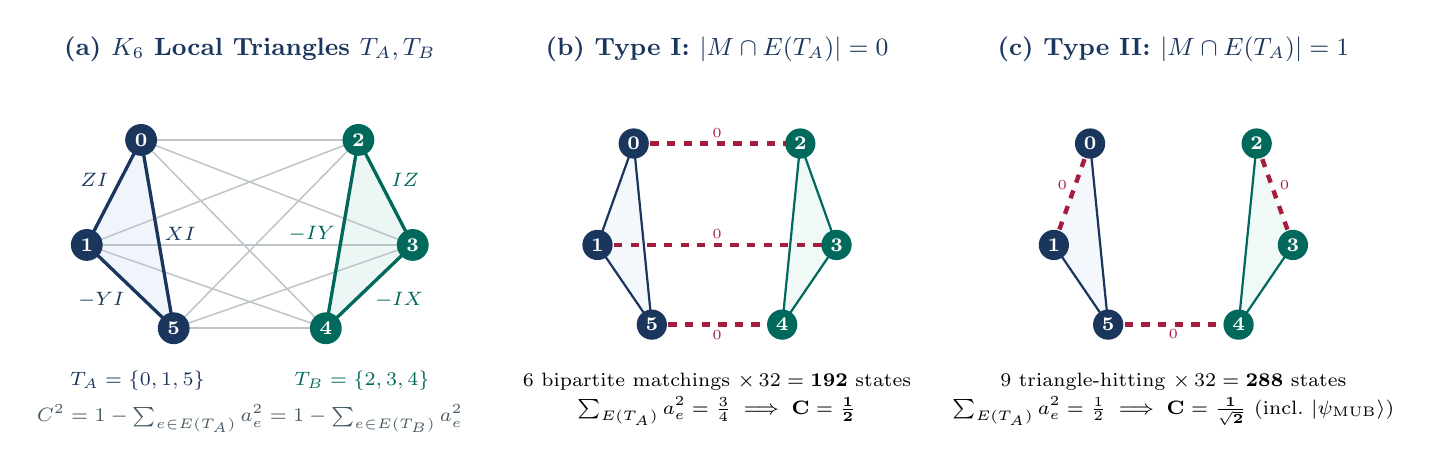
\begin{tikzpicture}[scale=0.92, every node/.style={font=\small}]
    % -------- LEFT PANEL: K_6 with Triangles T_A and T_B --------
    \begin{scope}[shift={(0,0)}]
      \node[font=\small\bfseries, text=Navy] at (0, 2.55) {(a) $K_6$ Local Triangles $T_A, T_B$};

      % Vertices of T_A (left triangle: 0, 1, 5)
      \coordinate (v0) at (-1.50, 1.30);
      \coordinate (v1) at (-2.25, -0.15);
      \coordinate (v5) at (-1.05, -1.30);
      % Vertices of T_B (right triangle: 2, 3, 4)
      \coordinate (v2) at (1.50, 1.30);
      \coordinate (v3) at (2.25, -0.15);
      \coordinate (v4) at (1.05, -1.30);

      % Shaded triangles
      \fill[LightBlue, opacity=0.75] (v0) -- (v1) -- (v5) -- cycle;
      \fill[LightTeal, opacity=0.75] (v2) -- (v3) -- (v4) -- cycle;

      % 9 nonlocal edges between T_A and T_B (light gray)
      \foreach \a in {v0,v1,v5} {
        \foreach \b in {v2,v3,v4} {
          \draw[Slate!35, line width=0.55pt] (\a) -- (\b);
        }
      }

      % T_A edges (blue)
      \draw[Navy, very thick] (v0) -- node[above left, font=\scriptsize, inner sep=1.5pt] {$ZI$} (v1);
      \draw[Navy, very thick] (v0) -- node[right, font=\scriptsize, inner sep=2pt] {$XI$} (v5);
      \draw[Navy, very thick] (v1) -- node[below left, font=\scriptsize, inner sep=1.5pt] {$-YI$} (v5);

      % T_B edges (teal)
      \draw[Teal, very thick] (v2) -- node[above right, font=\scriptsize, inner sep=1.5pt] {$IZ$} (v3);
      \draw[Teal, very thick] (v2) -- node[left, font=\scriptsize, inner sep=2pt] {$-IY$} (v4);
      \draw[Teal, very thick] (v3) -- node[below right, font=\scriptsize, inner sep=1.5pt] {$-IX$} (v4);

      % Nodes
      \foreach \p/\lbl in {v0/0, v1/1, v5/5} {
        \node[circle, fill=Navy, text=white, inner sep=1.8pt, font=\scriptsize\bfseries] at (\p) {\lbl};
      }
      \foreach \p/\lbl in {v2/2, v3/3, v4/4} {
        \node[circle, fill=Teal, text=white, inner sep=1.8pt, font=\scriptsize\bfseries] at (\p) {\lbl};
      }

      \node[font=\scriptsize\bfseries, text=Navy] at (-1.55, -2.02) {$T_A = \{0,1,5\}$};
      \node[font=\scriptsize\bfseries, text=Teal] at (1.55, -2.02) {$T_B = \{2,3,4\}$};
      \node[font=\scriptsize, text=Slate] at (0, -2.55) {$C^2 = 1 - \sum_{e \in E(T_A)} a_e^2 = 1 - \sum_{e \in E(T_B)} a_e^2$};
    \end{scope}

    % -------- MIDDLE PANEL: Type I Bipartite Matching (C = 1/2) --------
    \begin{scope}[shift={(6.45,0)}]
      \node[font=\small\bfseries, text=Navy] at (0, 2.55) {(b) Type I: $\lvert M \cap E(T_A)\rvert = 0$};

      \coordinate (a0) at (-1.15, 1.25);
      \coordinate (a1) at (-1.65, -0.15);
      \coordinate (a5) at (-0.90, -1.25);
      \coordinate (b2) at (1.15, 1.25);
      \coordinate (b3) at (1.65, -0.15);
      \coordinate (b4) at (0.90, -1.25);

      \fill[LightBlue, opacity=0.55] (a0) -- (a1) -- (a5) -- cycle;
      \fill[LightTeal, opacity=0.55] (b2) -- (b3) -- (b4) -- cycle;

      % Active edges in T_A and T_B (all 3 have |a_e| = 1/2)
      \draw[Navy, thick] (a0) -- (a1) -- (a5) -- cycle;
      \draw[Teal, thick] (b2) -- (b3) -- (b4) -- cycle;

      % Zero matching (3 bipartite edges, dashed crimson)
      \draw[Crimson, ultra thick, dashed] (a0) -- node[above, font=\tiny, text=Crimson, inner sep=1.5pt] {$0$} (b2);
      \draw[Crimson, ultra thick, dashed] (a1) -- node[above, font=\tiny, text=Crimson, inner sep=1.5pt] {$0$} (b3);
      \draw[Crimson, ultra thick, dashed] (a5) -- node[below, font=\tiny, text=Crimson, inner sep=1.5pt] {$0$} (b4);

      \foreach \p/\lbl in {a0/0, a1/1, a5/5} {
        \node[circle, fill=Navy, text=white, inner sep=1.6pt, font=\scriptsize\bfseries] at (\p) {\lbl};
      }
      \foreach \p/\lbl in {b2/2, b3/3, b4/4} {
        \node[circle, fill=Teal, text=white, inner sep=1.6pt, font=\scriptsize\bfseries] at (\p) {\lbl};
      }

      \node[font=\scriptsize, align=center] at (0, -2.28) {
        $6$ bipartite matchings $\times\, 32 = \mathbf{192}$ states\\[2pt]
        $\sum_{E(T_A)} a_e^2 = \tfrac{3}{4} \implies \mathbf{C = \tfrac{1}{2}}$
      };
    \end{scope}

    % -------- RIGHT PANEL: Type II Triangle-Hitting Matching (C = 1/sqrt(2)) --------
    \begin{scope}[shift={(12.75,0)}]
      \node[font=\small\bfseries, text=Navy] at (0, 2.55) {(c) Type II: $\lvert M \cap E(T_A)\rvert = 1$};

      \coordinate (c0) at (-1.15, 1.25);
      \coordinate (c1) at (-1.65, -0.15);
      \coordinate (c5) at (-0.90, -1.25);
      \coordinate (d2) at (1.15, 1.25);
      \coordinate (d3) at (1.65, -0.15);
      \coordinate (d4) at (0.90, -1.25);

      \fill[LightBlue, opacity=0.55] (c0) -- (c1) -- (c5) -- cycle;
      \fill[LightTeal, opacity=0.55] (d2) -- (d3) -- (d4) -- cycle;

      % Nonzero triangle edges
      \draw[Navy, thick] (c0) -- (c5) -- (c1);
      \draw[Teal, thick] (d2) -- (d4) -- (d3);

      % Zero matching of psi_MUB: (0,1), (2,3), (4,5)
      \draw[Crimson, ultra thick, dashed] (c0) -- node[above left, font=\tiny, text=Crimson, inner sep=1pt] {$0$} (c1);
      \draw[Crimson, ultra thick, dashed] (d2) -- node[above right, font=\tiny, text=Crimson, inner sep=1pt] {$0$} (d3);
      \draw[Crimson, ultra thick, dashed] (c5) -- node[below, font=\tiny, text=Crimson, inner sep=1pt] {$0$} (d4);

      \foreach \p/\lbl in {c0/0, c1/1, c5/5} {
        \node[circle, fill=Navy, text=white, inner sep=1.6pt, font=\scriptsize\bfseries] at (\p) {\lbl};
      }
      \foreach \p/\lbl in {d2/2, d3/3, d4/4} {
        \node[circle, fill=Teal, text=white, inner sep=1.6pt, font=\scriptsize\bfseries] at (\p) {\lbl};
      }

      \node[font=\scriptsize, align=center] at (0, -2.28) {
        $9$ triangle-hitting $\times\, 32 = \mathbf{288}$ states\\[2pt]
        $\sum_{E(T_A)} a_e^2 = \tfrac{1}{2} \implies \mathbf{C = \tfrac{1}{\sqrt{2}}}$ (incl.\ $\psimub$)
      };
    \end{scope}
  \end{tikzpicture}%
  }
  \caption{Geometric origin of the entanglement-magic dichotomy on $K_6$. (a) The $3$ local qubit-$A$ Paulis form the triangle $T_A = \{0,1,5\}$ and the $3$ local qubit-$B$ Paulis form the complementary triangle $T_B = \{2,3,4\}$. Dashed crimson edges indicate the $3$ vanishing Paulis (a perfect matching $M$) of a maximizer, while every non-matching edge has $\lvert a_e\rvert = 1/2$. (b) The $3! = 6$ bipartite matchings miss $T_A$ completely, giving $C = 1/2$ ($192$ states). (c) The remaining $3\times 3 = 9$ matchings contain $1$ edge in $T_A$ and $1$ edge in $T_B$ (illustrated for $\psimub$ with $M_0 = \{(0,1),(2,3),(4,5)\}$), giving $C = 1/\sqrt{2}$ ($288$ states).}
  \label{fig:k6-concurrence}
\end{figure}

Note how transparently \Cref{prop:conc-triangle} explains the impossibility of maximal entanglement ($C = 1$) or separability ($C = 0$): achieving $C = 1$ would require all $3$ edges of $E(T_A)$ to vanish simultaneously, which is impossible for a matching; achieving $C = 0$ would require $\sum_{e\in E(T_A)} a_e^2 = 1$, which is impossible because every edge has $a_e^2 \le 1/4$, capping the triangle sum at $3/4 < 1$.

\FloatBarrier

%==============================================================================
\section{Exact Equivariant SOS Construction and Witnessed Orbit Cancellation}
\label{sec:methodology}
%==============================================================================

While Sections~\ref{sec:so6}--\ref{sec:entanglement} establish all parts of \Cref{thm:main}, the exact degree-$8$ polynomial certificate of \Cref{thm:master-sos} requires reconciling two distinct goals: (i) discovering a compact, exact rational SOS decomposition on a variety whose optimum is attained on a $480$-point extremizer set, and (ii) verifying the resulting $\Bplus$-equivariant identity cleanly both in standalone exact arithmetic and inside Lean~4's pure type-checking kernel. In this section we position our construction relative to existing exact SOS literature, document the complete reproducible discovery pipeline, and present the orbit-cancellation witness lemma used for kernel verification.

\subsection{Bottlenecks and Relation to Prior Exact SOS Methods}

Consider the generic problem of proving a sharp lower bound
\begin{equation}
  \label{eq:gen-pop}
  f(x) \;\ge\; \gamma \qquad (\forall\, x \in V \subset \R^n),
\end{equation}
where $f \in \Q[x]$ and the real algebraic variety $V = \{x \in \R^n : \eta_1(x) = \cdots = \eta_m(x) = 0\}$ are invariant under a finite group $G$ acting on $\R^n$ by signed coordinate permutations, $(g \cdot x)_i = \varepsilon(g,i)\, x_{\hat{g}(i)}$ with $\varepsilon(g,i) \in \{\pm 1\}$ and $\hat{g} \in S_n$.

\begin{enumerate}[label=\textbf{Bottleneck \arabic*:}, leftmargin=*, itemsep=4pt]
  \item \textbf{Singular Gram matrices at sharp bounds.} Numerical Lasserre/Parrilo SDP solvers~\cite{Lasserre2001,Parrilo2003} produce floating-point Gram matrices $\Gamma_{\mathrm{num}} \succeq 0$. Certification tactics based on floating-point perturbation/padding and verified Cholesky factorization---such as \textsc{ValidSDP}~\cite{MartinDorelRoux2017,Roux2018}---require $\Gamma_{\mathrm{num}}$ to be \emph{strictly positive definite} so that a small norm perturbation absorbs rounding errors. Whenever $\gamma$ is the \emph{exact} minimum attained on a nonempty extremizer set $V^{\max} \subset V$, every valid SOS Gram matrix must vanish on the monomial evaluations at $V^{\max}$ and is therefore necessarily \emph{rank-deficient} (singular); padding-based tactics can then certify only a loose bound $\gamma - \varepsilon$, not the sharp constant $\gamma$ or its extremizers. In exact polynomial optimization, this singularity is addressed by combining \emph{facial reduction}~\cite{PermenterParrilo2018} with symmetry reduction~\cite{GatermannParrilo2004,Riener2013} and exact rational projection or rounding~\cite{PeyrlParrilo2008,Kaltofen2008,Kaltofen2012,MagronSafeyElDin2018}.
  \item \textbf{Symmetrization overhead in pure-kernel proof assistants.} Even after exact rational polynomials $Q_k, L_\ell$ are recovered for an un-symmetrized seed $F$, certifying the Reynolds-operator identity $\sum_{h\in G} F(h\cdot x) \equiv 0$ inside a proof assistant's kernel is nontrivial. Naive averaging over all $\lvert G\rvert$ group elements requires $O(\lvert G\rvert \cdot \lvert F\rvert)$ monomial actions---here $23{,}040 \times 1{,}409 \approx 3.25 \times 10^7$. Exploiting the semidirect product $\Bplus = (\Z/2\Z)^5 \rtimes S_6$ eliminates the diagonal sign subgroup via a vertex-degree parity filter, reducing the summation to $\lvert S_6\rvert \cdot \lvert F\rvert = 720 \times 1{,}409 \approx 1.01 \times 10^6$ monomial actions (which executes in under a second in Python), but even $10^6$ polynomial actions would be expected to incur substantial overhead under pure definitional reduction (\code{rfl}) inside Lean~4's kernel and would require formalizing group-specific decomposition lemmas.
\end{enumerate}

\subsection{Reproducible Certificate Discovery Pipeline}

All discovery scripts and exact intermediate artifacts are included in \code{scripts/} in the accompanying repository and reproduce \code{CertificateData.lean} byte-for-byte with zero external numerical libraries (\Cref{fig:cert-pipeline}). Throughout the pipeline, let $N_{\mathrm{sign}} := \{(\mathrm{id}, s) \in \Bplus : \prod_{i=0}^5 s_i = +1\} \cong (\Z/2\Z)^5$ denote the normal even-sign subgroup of order $32$, and fix the $720$-element coset transversal
\begin{equation}
  \label{eq:transversal}
  \mathcal{T} \;:=\; \bigl\{\, (p, s_0(p)) \in \Bplus \;:\; p \in S_6 \,\bigr\},
  \qquad s_0(p) := (\sgn(p), 1, 1, 1, 1, 1),
\end{equation}
representing the quotient $\Bplus / N_{\mathrm{sign}} \cong S_6$ (note that $\mathcal{T}$ is a complete set of coset representatives rather than a subgroup). Because $N_{\mathrm{sign}} \trianglelefteq \Bplus$ is normal, any $N_{\mathrm{sign}}$-invariant polynomial $P$ satisfies $\sum_{h\in\Bplus} P(h\cdot a) = 32 \sum_{t\in\mathcal{T}} P(t\cdot a)$; thus averaging over $\mathcal{T}$ reproduces the full $\Bplus$-average. The pipeline proceeds in five stages (matching the five scripts in \code{scripts/}, grouped into three blocks in \Cref{fig:cert-pipeline}), all strictly outside the trusted computing base:

\begin{figure}[t]
  \centering
  \resizebox{\textwidth}{!}{%
  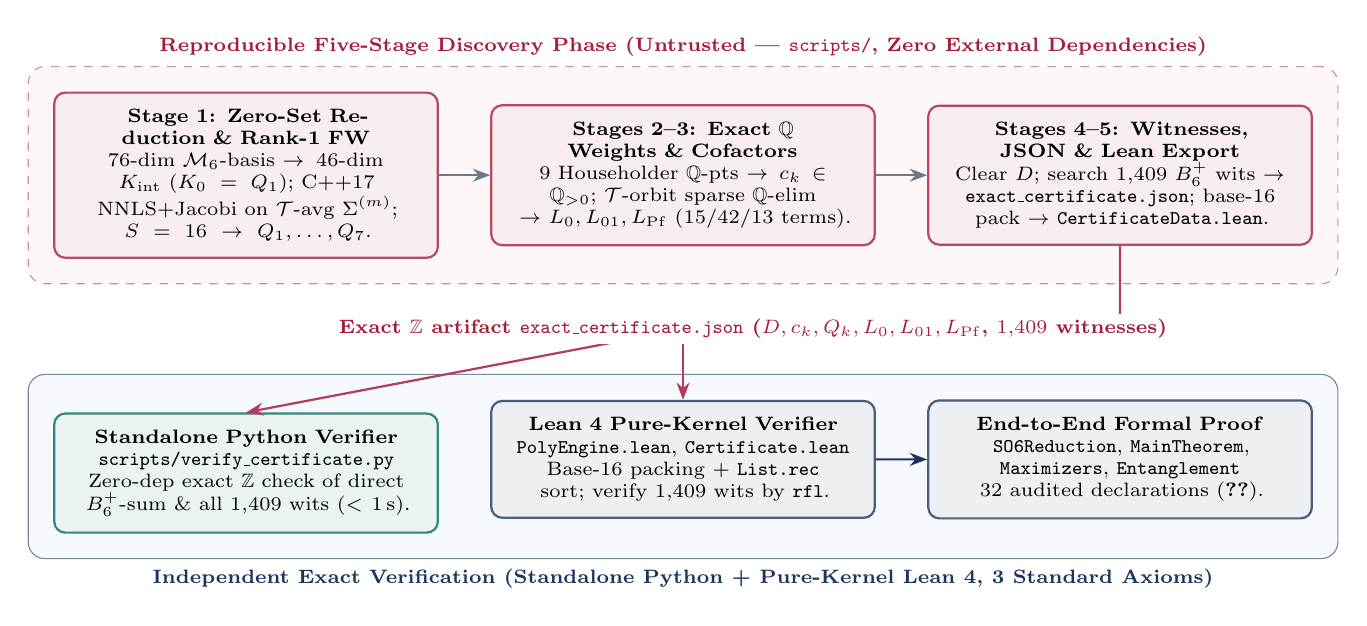
\begin{tikzpicture}[
    node distance=0.55cm and 0.65cm,
    box/.style={rectangle, rounded corners=4pt, draw=#1!80, fill=#1!8, thick,
                text width=4.45cm, align=center, inner sep=6pt, font=\scriptsize},
    arrow/.style={-{Stealth[length=2.2mm]}, thick, Slate!80}
  ]
    % Discovery phase (top row)
    \node[box=Crimson] (s1) {\textbf{Stage 1: Zero-Set Reduction \& Rank-1 FW}\\
      $76$-dim $\Mman$-basis $\to 46$-dim $K_{\mathrm{int}}$ ($K_0=Q_1$); C++17 NNLS+Jacobi on $\mathcal{T}$-avg $\Sigma^{(m)}$; $S=16 \to Q_1,\dots,Q_7$.};
    \node[box=Crimson, right=of s1] (s2) {\textbf{Stages 2--3: Exact $\Q$ Weights \& Cofactors}\\
      $9$ Householder $\Q$-pts $\to c_k \in \Q_{>0}$; $\mathcal{T}$-orbit sparse $\Q$-elim $\to L_0, L_{01}, L_{\mathrm{Pf}}$ ($15/42/13$ terms).};
    \node[box=Crimson, right=of s2] (s3) {\textbf{Stages 4--5: Witnesses, JSON \& Lean Export}\\
      Clear $D$; search $1{,}409$ $\Bplus$ wits $\to$ \texttt{exact\_certificate.json}; base-$16$ pack $\to$ \texttt{CertificateData.lean}.};

    % Verification phase (bottom row)
    \node[box=Teal, below=1.95cm of s1] (k1) {\textbf{Standalone Python Verifier}\\
      \texttt{scripts/verify\_certificate.py}\\
      Zero-dep exact $\Z$ check of direct $\Bplus$-sum \& all $1{,}409$ wits ($<1\,\mathrm{s}$).};
    \node[box=Navy, below=1.95cm of s2] (k2) {\textbf{Lean~4 Pure-Kernel Verifier}\\
      \texttt{PolyEngine.lean}, \texttt{Certificate.lean}\\
      Base-$16$ packing + \texttt{List.rec} sort; verify $1{,}409$ wits by \texttt{rfl}.};
    \node[box=Navy, below=1.95cm of s3] (k3) {\textbf{End-to-End Formal Proof}\\
      \texttt{SO6Reduction}, \texttt{MainTheorem}, \texttt{Maximizers}, \texttt{Entanglement}\\
      $32$ audited declarations (\Cref{app:lean}).};

    % Background containers
    \begin{scope}[on background layer]
      \node[fit=(s1)(s2)(s3), draw=Crimson!50, dashed, rounded corners=6pt, fill=LightRed!45,
            inner sep=9pt, label={[font=\scriptsize\bfseries, text=Crimson]above:Reproducible Five-Stage Discovery Phase (Untrusted --- \texttt{scripts/}, Zero External Dependencies)}] (topbox) {};
      \node[fit=(k1)(k2)(k3), draw=Navy!60, rounded corners=6pt, fill=LightBlue!45,
            inner sep=9pt, label={[font=\scriptsize\bfseries, text=Navy]below:Independent Exact Verification (Standalone Python + Pure-Kernel Lean~4, 3 Standard Axioms)}] (botbox) {};
    \end{scope}

    % Arrows
    \draw[arrow] (s1) -- (s2);
    \draw[arrow] (s2) -- (s3);
    \coordinate (midy) at ($(topbox.south)!0.5!(botbox.north)$);
    \draw[arrow, Crimson!85, thick] (s3.south) |- (midy) -- (k1.north);
    \draw[arrow, Crimson!85, thick] (midy -| k2.north) -- (k2.north);
    \node[font=\scriptsize\bfseries, text=Crimson, fill=white, inner sep=2pt]
      at ($(midy -| s3.south)!0.42!(midy -| k1.north)$)
      {Exact $\Z$ artifact \texttt{exact\_certificate.json} ($D, c_k, Q_k, L_0, L_{01}, L_{\mathrm{Pf}}$, $1{,}409$ witnesses)};
    \draw[arrow, Navy] (k2) -- (k3);
  \end{tikzpicture}%
  }
  \caption{Reproducible five-stage discovery and independent verification architecture for \Cref{thm:master-sos}. All numerical optimization, integer rounding, exact rational solves, witness search, and Lean~4 export (in \code{scripts/}) occur outside the trusted computing base and produce \code{scripts/\allowbreak exact\_certificate.json}, which is verified both directly in Python and inside Lean~4's pure kernel (\Cref{app:lean}).}
  \label{fig:cert-pipeline}
\end{figure}

\paragraph{Stage 1: Zero-set face restriction and rank-$1$ Frank--Wolfe SDP.}
Because $Q_1(a) = 4a_0^3 - a_0$ transforms under $N_{\mathrm{sign}}$ by the one-dimensional character $\chi_{(0,1)}(s) = s_0 s_1 = s_2 s_3 s_4 s_5$, the C++17 program \code{extract\_int\_cert.cpp} restricts the SOS ansatz to degree-$\le 4$ monomials with vertex-parity masks $\{0,1\}$ or $\{2,3,4,5\}$ (so every square $Q_k(a)^2$ is $N_{\mathrm{sign}}$-invariant). Evaluating these monomials on $250$ random points of $\Mman$ and applying Gram--Schmidt orthogonalization in ascending degree order selects $76$ linearly independent monomials on $\Mman$. We then restrict the Gram basis to the face of the PSD cone determined by the extremizer set $\Mman^{\max}$ (zero-set reduction, in the spirit of facial reduction~\cite{PermenterParrilo2018}): computing the reduced row-echelon form of the $480 \times 76$ evaluation matrix on $\Mman^{\max}$ yields a $46$-dimensional nullspace whose free-column basis clears denominators by divisors of $24$, giving an exact $46$-dimensional sparse integer basis $K_{\mathrm{int}}$ vanishing identically on $\Mman^{\max}$ with $K_0 = Q_1 = 4a_0^3 - a_0$.

Rather than forming a dense $46 \times 46$ Gram matrix and taking a high-rank $LDL^T$ factorization, we sample $12$ points on $\Mman$ ($J_0$ plus $11$ random orthogonal complex structures), form the $\mathcal{T}$-averaged $46 \times 46$ moment matrices $\Sigma^{(m)}$ ($m = 0,\dots,11$), reserve an initial weight $\varepsilon_0 = 0.02$ on $K_0 = Q_1$, and run a zero-dependency primal-dual \emph{rank-$1$ Frank--Wolfe} (simplicial decomposition) solver on the remaining target. Each outer iteration solves an active-set non-negative least-squares master problem (Lawson--Hanson NNLS) over the collected rank-$1$ rays and calls a cyclic Jacobi eigensolver on $\sum_m \mathrm{res}_m \Sigma^{(m)}$ to add the most violated rank-$1$ ray, with no identity-matrix padding. The solver converges in $27$ iterations (relative residual $1.84 \times 10^{-14}$) to $8$ active rank-$1$ vectors; because the squares are subsequently averaged over $\Bplus$, the individual seed polynomials $Q_k$ need not be invariant under the edge stabilizer $S_2 \times S_4$. Rounding the active vectors in the $K_{\mathrm{int}}$ basis at integer scales $S \in \{8, 10, 12\}$ also achieves NNLS relative residuals below $9 \times 10^{-15}$ on an unreserved NNLS re-solve, but drives the weight on $Q_1$ to zero; $S = 16$ is the smallest tested scale that preserves a strictly positive weight on $Q_1$ (yielding $c_1/D \approx 1.10 \times 10^{-3} > 0$, essential for \Cref{cor:so6-eq}, in place of the temporary discovery bias $\varepsilon_0 = 0.02$). Dividing each expanded polynomial by its coefficient GCD leaves $7$ active sparse integer polynomials $Q_1, \dots, Q_7 \in \Z[a_0,\dots,a_{14}]$ ($\max\lvert\text{coeff}\rvert \le 384$, NNLS relative residual $5.62 \times 10^{-14}$).

\paragraph{Stage 2: Exact rational weights.}
In \code{verify\_exact\_Q.py}, to recover exact rational weights $c_1, \dots, c_7 \in \Q_{>0}$ without floating-point rounding, we construct $9$ exact rational points $A \in \Mman(\Q)$ by conjugating $J_0$ with pairs of integer Householder reflections $H_{v_2} H_{v_1} \in \SO(6,\Q)$. Solving the $7\times 7$ exact rational linear system on the first $7$ points (with $\mathcal{T}$-averaged evaluations) yields strictly positive rational weights $c_1, \dots, c_7 \in \Q_{>0}$ whose residual vanishes identically on the $2$ held-out rational points.

\paragraph{Stage 3: Exact rational ideal cofactors.}
In \code{compute\_cofactors.py}, every monomial in $(15 a_0^4 - 3/4) - \sum_{k=1}^7 c_k Q_k(a)^2$ and in the candidate ideal multiples (degree-$\le 6$ multiples of $\eta_0, \eta_{01}, \zeta_{01}$ with matching vertex-parity masks) is $N_{\mathrm{sign}}$-invariant, so its signed $\Bplus$-orbit is exhausted by $\mathcal{T}$. Compressing the target modulo $\mathcal{T}$ produces $78$ nonzero canonical orbits of degree $\le 8$; sparse exact Gaussian elimination over $\Q$ against the $\mathcal{T}$-compressed ideal columns (ordered by $(\text{degree}, \text{nnz})$ to promote sparsity) terminates with zero remainder, producing rational cofactors $L_0$ ($15$ terms), $L_{01}$ ($42$ terms), and $L_{\mathrm{Pf}}$ ($13$ terms).

\paragraph{Stage 4: Denominator clearing, witness search, and JSON export.}
Clearing the least common denominator $D$ (a $29$-digit integer divisible by $4$) in \code{build\_witness\_table.py} yields exact integer weights $c_k \in \Z_{>0}$, integer cofactors, and the $1{,}409$-term integer remainder $F(a)$ of~\eqref{eq:seed-F}. Scanning the $720$ coset representatives in $\mathcal{T}$ (which suffices because every monomial of $F$ is $N_{\mathrm{sign}}$-invariant) assigns to every monomial of $F$ an explicit $\Bplus$ orbit-cancellation witness as formulated below, exporting the complete self-contained certificate to \code{scripts/exact\_certificate.json} ($124\,\mathrm{KB}$).

\paragraph{Stage 5: Lean~4 packing and data generation.}
Finally, \code{gen\_lean\_cert.py} packs every monomial into base-$16$ natural numbers, re-verifies the packed assembly and witness alignment, and emits \code{TwoQubitMaximalMagic/\allowbreak CertificateData.lean} byte-for-byte.

\subsection{Witnessed Orbit Cancellation for Proof-Kernel Verification}

To certify $\sum_{h\in G} F(h\cdot x) \equiv 0$ inside a proof assistant's pure kernel without iterating over $G$ or formalizing group-specific decompositions, we record the standard orbit-summation property of the Reynolds operator in an explicitly witnessed form:

\begin{lemma}[Witnessed Orbit Cancellation]
\label{lem:orbit-cancel}
Let $G$ be any finite group acting on $\R^n$ on the left by signed coordinate permutations, inducing the pullback (substitution) map on monomials $(g^* x^m)(x) := (g\cdot x)^m = \sigma(g, m)\, x^{\tau(g,m)}$ with $\sigma(g,m) \in \{\pm 1\}$. Let $F(x) = \sum_{j=1}^N \alpha_j x^{m_j} \in \Z[x_1,\dots,x_n]$ be a sparse polynomial with $N$ terms. Suppose each term $j \in \{1,\dots,N\}$ is annotated with one of two explicit witnesses:
\begin{enumerate}[label=\textup{(\alph*)}, leftmargin=2em]
  \item \textbf{Self-canceling witness} \textup{(\code{zero})}: an element $g_j \in G$ satisfying $g_j^* x^{m_j} = -x^{m_j}$;
  \item \textbf{Canonical-transfer witness} \textup{(\code{canon})}: a triple $(g_j, s_j, m_j^*)$ with $g_j \in G$, $s_j \in \{\pm 1\}$, and a canonical monomial $m_j^*$ satisfying $g_j^* x^{m_j} = s_j\, x^{m_j^*}$.
\end{enumerate}
Let $J_{\mathrm{canon}} \subseteq \{1,\dots,N\}$ be the set of indices carrying a \code{canon} witness. If the accumulated canonical polynomial vanishes identically,
\begin{equation}
  \label{eq:canon-cancel}
  \sum_{j \in J_{\mathrm{canon}}} (s_j \alpha_j)\, x^{m_j^*} \;\equiv\; 0 \qquad \text{in } \Z[x_1,\dots,x_n],
\end{equation}
then the $G$-symmetrization of $F$ vanishes identically on all of $\R^n$:
\begin{equation}
  \label{eq:orbit-cancel-conc}
  \sum_{h \in G} F(h \cdot x) \;\equiv\; 0 \qquad (\forall\, x \in \R^n).
\end{equation}
\end{lemma}

\begin{proof}
By linearity, $\sum_{h\in G} F(h\cdot x) = \sum_{j=1}^N \alpha_j \sum_{h\in G} (h\cdot x)^{m_j}$. Because left multiplication $h \mapsto g_j h$ is a bijection on $G$ and $(g_j h \cdot x)^{m_j} = (g_j \cdot (h\cdot x))^{m_j} = (g_j^* x^{m_j})(h\cdot x)$:
\begin{itemize}[leftmargin=1.8em, itemsep=2pt]
  \item For every $j$ with a \code{zero} witness,
  \[
    \sum_{h\in G} (h\cdot x)^{m_j}
    \;=\; \sum_{h\in G} (g_j h \cdot x)^{m_j}
    \;=\; \sum_{h\in G} (g_j^* x^{m_j})(h\cdot x)
    \;=\; -\sum_{h\in G} (h\cdot x)^{m_j},
  \]
  forcing $\sum_{h\in G} (h\cdot x)^{m_j} = 0$.
  \item For every $j \in J_{\mathrm{canon}}$,
  \[
    \alpha_j \sum_{h\in G} (h\cdot x)^{m_j}
    \;=\; \alpha_j \sum_{h\in G} (g_j h \cdot x)^{m_j}
    \;=\; \alpha_j \sum_{h\in G} (g_j^* x^{m_j})(h\cdot x)
    \;=\; (s_j \alpha_j) \sum_{h\in G} (h\cdot x)^{m_j^*}.
  \]
\end{itemize}
Substituting both identities yields $\sum_{h\in G} F(h\cdot x) = \sum_{h\in G} \bigl(\sum_{j\in J_{\mathrm{canon}}} (s_j \alpha_j)(h\cdot x)^{m_j^*}\bigr) = 0$ by~\eqref{eq:canon-cancel}.
\end{proof}

\begin{remark}[Complexity and Completeness]
Checking the hypotheses of \Cref{lem:orbit-cancel} requires verifying one group-element action per monomial ($O(N)$ work) followed by sorting and combining like terms in~\eqref{eq:canon-cancel} ($O(N\log N)$ work), independent of $\lvert G\rvert$. In our two-qubit certificate, $N = 1{,}409$ ($274$ \code{zero} witnesses and $1{,}135$ \code{canon} witnesses mapping onto $77$ canonical orbit representatives). This yields a $\sim 2.2\times 10^3$ work reduction ($\lvert\Bplus\rvert/\log_2 N$) relative to generic $\Bplus$-averaging ($23{,}040 \times 1{,}409 \approx 3.25\times 10^7$ actions), and a $\sim 70\times$ reduction ($\lvert S_6\rvert/\log_2 N$, or $720\times$ fewer group evaluations) even relative to the parity-reduced $S_6$ baseline ($720 \times 1{,}409 \approx 1.01\times 10^6$ actions, obtained by factoring out the diagonal sign subgroup $(\Z/2\Z)^5$), while remaining group-agnostic inside the proof kernel. The converse of \Cref{lem:orbit-cancel} holds as well: whenever $\sum_{h\in G} F(h\cdot x) \equiv 0$ under a signed-permutation group $G$, every monomial in $\mathrm{supp}(F)$ either admits an odd stabilizer element (a \code{zero} witness) or lies in an orientation-consistent orbit whose signed coefficient sum vanishes (yielding \code{canon} witnesses onto any chosen orbit representative). Thus the witness representation is both sound and complete.
\end{remark}

We provide two independent exact verifications of \Cref{thm:master-sos} and the full proof:
\begin{enumerate}[label=\arabic*., leftmargin=1.8em, itemsep=2pt]
  \item \textbf{Standalone zero-dependency Python check (\Cref{app:explicit}):} The $149$-line script \code{scripts/\allowbreak verify\_\allowbreak certificate.py} reads \code{scripts/\allowbreak exact\_\allowbreak certificate.json} and independently verifies in exact integer arithmetic (in under $1\,\mathrm{s}$, without Lean) both direct parity-reduced $\Bplus$ symmetrization $\sum_{h\in\Bplus} F(h\cdot a) \equiv 0$ and all $1{,}409$ orbit-cancellation witnesses.
  \item \textbf{Pure-kernel Lean~4 formalization (\Cref{app:lean}):} All $6$ parts of \Cref{thm:main} (from the raw definition of Pauli matrices and $M_\alpha$ through \Cref{thm:master-sos}, \Cref{thm:all-alpha}, \Cref{thm:480}, \Cref{thm:mub-equiv}, and \Cref{thm:concurrence}) are formally machine-checked inside Lean~4~\cite{deMouraUllrich2021,Mathlib2020} using pure definitional equality (\code{rfl}), with zero \code{sorry}, zero \code{native\_decide}, and only Lean's three standard foundational axioms.
\end{enumerate}

%==============================================================================
\section{Discussion, Open Problems, and Outlook}
\label{sec:discussion}
%==============================================================================

Our resolution of the two-qubit maximal magic conjecture completes the analytical picture for $n = 2$ qubits across the monotonicity regime $\alpha \ge 2$ and clarifies several open directions.

\paragraph{Higher-qubit, sub-$\alpha=2$, and bipartite qudit regimes of Open Quantum Problem E28.}
While $n = 1$ (tetrahedron WH-SIC), $n = 2$ (this work, $480$ Pauli $5$-MUB fiducial states), and $n = 3$ (Hoggar lines WH-SIC~\cite{Hoggar1998}) are now settled at the level of maximal pure-state SRE for $\alpha \ge 2$, several regimes remain open~\cite{LiuLowYin2026,OpenQuantumE28}:
\begin{itemize}[leftmargin=1.8em, itemsep=2pt]
  \item For $n = 3$ qubits ($d = 8$), the $\Pauli_3$-covariant Hoggar-line SIC-POVM saturates the WH-SIC bound $M_\alpha^{\mathrm{SIC}}(8)$ (with $M_2^{\mathrm{SIC}}(8) = \ln(9/2)$)~\cite{CuffaroFuchs2024}. Thus $n = 2$ is the smallest multi-qubit dimension where the Pauli group fails to support a SIC-POVM and maximal magic drops strictly below $M_\alpha^{\mathrm{SIC}}$.
  \item For $n \ge 4$ qubits ($d = 2^n \ge 16$), Godsil and Roy~\cite{GodsilRoy2009} proved that---just as for $n = 2$---no $\Pauli_n$-covariant SIC-POVM exists; Liu, Low, and Yin~\cite{LiuLowYin2026} conjectured that Pauli MUB fiducial states continue to maximize $M_2$ for all $n \neq 1, 3$. Proving or disproving this conjecture for $n = 4$ is the next major multi-qubit frontier of Problem~E28.
  \item In the non-monotone regime $0 < \alpha < 2$, the $\alpha = 2$ moment lower bound of \Cref{cor:so6-eq} no longer bounds the $2\alpha$-moment from below. Indeed, numerical results reported in~\cite{LiuLowYin2026,OpenQuantumE28} indicate that a different family of two-qubit states overtakes the $480$ Pauli $5$-MUB fiducials as maximizers of $M_\alpha$ for $\alpha < 1.64$, leaving the intermediate range $\alpha \in [\approx 1.64, 2)$ open. Extending sharp bounds to \emph{mixed} two-qubit states via the convex-roof SRE~\cite{LeoneBittel2024} and rigorously proving global optimality along the full two-qubit magic--entanglement Pareto frontier of Roman et al.~\cite{Roman2026} are also natural follow-up problems.
  \item Beyond qubits, Knipfer, Roman, Matcheva, and Matchev~\cite{Knipfer2026} recently analyzed bipartite qudit systems, finding numerical and analytical evidence for a maximal second-order SRE of $M_2 = \ln(81/17)$ for two qutrits ($d=3$, attained at $18$ Weyl--Heisenberg MUB fiducial spectra) and $M_2 = \ln(625/49)$ for two ququints ($d=5$), and conjecturing $\max M_2 = \ln[d^4/(2d^2-1)]$ for pairs of prime-dimensional qudits. Certifying the two-qutrit bound $\ln(81/17)$ algebraically is an appealing next target for symmetry-reduced exact SOS methods.
\end{itemize}

\paragraph{Scope and computational bottlenecks for larger quantum symmetries.}
Our certification pipeline illustrates both the strengths and the practical limits of exact equivariant SOS proofs in quantum information. Witnessed orbit cancellation (\Cref{lem:orbit-cancel}) removes the dependence on $\lvert G\rvert$ during \emph{formal verification}, making kernel checking feasible even when $\lvert G\rvert$ is large. For larger multi-qubit systems such as $n = 4$ ($4^4 - 1 = 255$ non-identity Pauli coordinates), however, the dominant computational bottleneck lies in the \emph{certificate discovery phase}: constructing a tractable symmetry-reduced SDP over $255$ variables and keeping the monomial support $\lvert F\rvert$ of the resulting exact certificate manageable. By contrast, lower-dimensional symmetric problems with compact algebraic parameterizations---such as two-qutrit magic bounds~\cite{Knipfer2026}, tight Bell and Tsirelson inequalities with permutation symmetry, stabilizer-polytope facets, and polynomial invariants of two-qubit entanglement~\cite{Makhlin2002}---fall well within the practical reach of zero-set face restriction, rank-$1$ Frank--Wolfe discovery, and witnessed pure-kernel certification.

%==============================================================================
\section*{Acknowledgments}
%==============================================================================
The author thanks the Lean~4 and Mathlib communities for the open-source verification infrastructure that enabled pure-kernel certification of this proof, and acknowledges Qiaofeng Liu, Ian Low, and Zhewei Yin for formulating the two-qubit maximal magic conjecture and Open Quantum Problem~E28 that motivated this work.

%==============================================================================
\appendix
\section{Explicit Clifford Generators and Standalone Certificate Verification}
\label{app:explicit}
%==============================================================================

\subsection{Explicit \texorpdfstring{$4\times 4$}{4x4} Clifford Generators Realizing \texorpdfstring{$\Bplus$}{B6+}}
From \Cref{prop:clifford-lift} and \Cref{tab:k6-dict}, the five $\pi/2$ Pauli-rotation unitaries $U_k = \frac{1}{\sqrt{2}}(I_4 + i\tilde{P}_{e_k})$ generating $\PCl_2 \cong \PBplus$ on $\Mman$ are explicitly:
\begin{align*}
  U_0 &= \tfrac{1}{\sqrt{2}}(I_4 + i\, ZI) = \mathrm{diag}(e^{i\pi/4}, e^{i\pi/4}, e^{-i\pi/4}, e^{-i\pi/4}), \\
  U_1 &= \tfrac{1}{\sqrt{2}}(I_4 - i\, XX), \qquad
  U_2 = \tfrac{1}{\sqrt{2}}(I_4 + i\, IZ), \\
  U_3 &= \tfrac{1}{\sqrt{2}}(I_4 - i\, IX), \qquad
  U_4 = \tfrac{1}{\sqrt{2}}(I_4 + i\, ZZ).
\end{align*}
Together, $U_0, U_2, U_3$ are single-qubit Clifford gates while $U_1, U_4$ are maximally entangling two-qubit Clifford rotations.

\subsection{Machine-Readable Certificate, Discovery Scripts, and Standalone Verifier}
To allow readers without Lean~4 to inspect $Q_1, \dots, Q_7$, $c_1, \dots, c_7$, $D$, and the ideal cofactors $L_0, L_{01}, L_{\mathrm{Pf}}$ directly and reproduce both discovery and verification, the repository (release tag \code{v1.0})
\begin{center}
  \url{https://github.com/LingyeNBird/two-qubit-maximal-magic}
\end{center}
includes a self-contained \code{scripts/} directory requiring only a C++17 compiler and the Python~3 standard library:
\begin{itemize}[leftmargin=1.8em, itemsep=2pt]
  \item \code{scripts/exact\_certificate.json} ($124\,\mathrm{KB}$): complete exact integer certificate ($D$, $c_1,\dots,c_7$, $Q_1,\dots,Q_7$, $L_0, L_{01}, L_{\mathrm{Pf}}$, and all $1{,}409$ $\Bplus$ witnesses).
  \item \code{scripts/verify\_certificate.py}: standalone exact-integer verifier ($149$ lines, $< 1\,\mathrm{s}$) checking $D > 0$, $4\mid D$, $c_k > 0$, $Q_1 = 4a_0^3 - a_0$, exact expansion of $F(a)$, direct parity-reduced $\Bplus$ symmetrization $\sum_{h\in\Bplus} F(h\cdot a) \equiv 0$, and all $1{,}409$ explicit witnesses.
  \item Five-stage discovery pipeline in \code{scripts/} reproducing the JSON and Lean~4 certificates byte-for-byte:
  \begin{enumerate}[label=\arabic*., leftmargin=1.6em, itemsep=1pt, topsep=2pt]
    \item \code{extract\_int\_cert.cpp}: zero-set face restriction ($76 \to 46$ dim) and rank-$1$ Frank--Wolfe SDP yielding $Q_1, \dots, Q_7$;
    \item \code{verify\_exact\_Q.py}: Householder $\Q$-point solve for exact weights $c_1, \dots, c_7 \in \Q_{>0}$;
    \item \code{compute\_cofactors.py}: sparse $\Q$-elimination for zero-remainder cofactors $L_0, L_{01}, L_{\mathrm{Pf}}$;
    \item \code{build\_witness\_table.py}: denominator clearing ($D$), witness search, and JSON export;
    \item \code{gen\_lean\_cert.py}: base-$16$ packing and byte-for-byte emission of \code{CertificateData.lean}.
  \end{enumerate}
\end{itemize}

%==============================================================================
\section{Lean~4 Pure-Kernel Implementation and Audited Theorem Index}
\label{app:lean}
%==============================================================================

\subsection{Pure-Kernel Engineering in Lean~4}
We implemented the complete end-to-end proof---from the raw definition of two-qubit Pauli matrices and Stabilizer R\'enyi Entropy to all $6$ parts of \Cref{thm:main}---in Lean~4 (\code{v4.36.0} + Mathlib4)~\cite{deMouraUllrich2021,Mathlib2020}, avoiding \code{sorry}, custom axioms, and compiler-trusting tactics such as \code{native\_decide}. Three engineering choices make pure-kernel (\code{rfl}) verification of \Cref{lem:orbit-cancel} practical inside Lean's type-checking kernel (reproducible via \code{lake build \&\& lake env lean Audit.lean}; \Cref{tab:lean-modules}):

\begin{enumerate}[label=\arabic*., leftmargin=1.8em, itemsep=2pt]
  \item \textbf{Base-$16$ bit-packed monomials:} Each degree-$\le 8$ monomial $\prod_{e=0}^{14} a_e^{d_e}$ is packed into a single natural number $m = \sum_{e=0}^{14} d_e \cdot 16^e < 16^{15}$ ($60$ bits). Monomial multiplication reduces to a single integer addition $m_1 + m_2$, proved unconditionally sound whenever a Boolean guard confirms $\max_e(d_e(m_1) + d_e(m_2)) < 16$ (carry-free digits).
  \item \textbf{Pure structural-recursion merge sort (\code{List.rec}):} Standard well-founded sorting in Lean generates heavy \code{WellFounded.fix} proof terms that stall kernel reduction. We implemented a fuel-bounded merge sort (\code{msortPoly}) and adjacent-term combiner (\code{combineAdj}) purely by structural recursion on \code{Nat} and \code{List}, proving unconditional evaluation preservation (\code{evalPoly (normPoly p) a = evalPoly p a}) so normalization reduces directly by \code{rfl} in the kernel.
  \item \textbf{Computable witness lifting:} Each witness $g_j \in \Bplus$ is stored as a flat record \code{B6Wit} of $6$ vertex images and $6$ Booleans checked by a Boolean validity predicate \code{isValidB6Wit}, which lifts formally into the mathematical group $\Bplus$. Checking all $1{,}409$ witnesses and the cancellation of all $77$ canonical orbit sums reduces to $15$ chunked witness \code{rfl} lemmas plus $1$ canonical-cancellation \code{rfl} lemma verified inside Lean's kernel.
\end{enumerate}

\begin{table}[htbp]
  \centering
  \caption{Module-by-module summary of the Lean~4 formalization (\code{v4.36.0} + Mathlib4). Every exported declaration in \code{Audit.lean} depends strictly on Lean's three standard axioms \code{[propext, Classical.choice, Quot.sound]} with zero \code{sorry} and zero \code{native\_decide}.}
  \label{tab:lean-modules}
  \footnotesize
  \begin{tabularx}{\textwidth}{@{}lrr>{\raggedright\arraybackslash}X@{}}
    \toprule
    Lean Module & Lines & Audited & Mathematical Content \\
    \midrule
    \code{Defs.lean}            & $236$   & ---  & Pure states, $\Pauli_2$, $\expval{\psi}{P}$, $M_\alpha$ \\
    \code{SO6Reduction.lean}    & $1{,}170$ & ---  & $\Mman$, $\Phi(A)=8A$, $\Bplus$ action, \Cref{prop:so6-embed}(a,b) \\
    \code{PolyEngine.lean}      & $722$   & ---  & Base-$16$ sparse engine, \code{List.rec} sort, \Cref{lem:orbit-cancel} \\
    \code{CertificateData.lean} & $2{,}459$ & ---  & Exact $D, c_k, Q_k, L_0, L_{01}, L_{\mathrm{Pf}}$, $1{,}409$ $\Bplus$ witnesses \\
    \code{Certificate.lean}     & $418$   & $3$  & Pure-kernel \code{rfl} SOS proof, \Cref{thm:master-sos} and \Cref{cor:so6-eq} \\
    \code{MainTheorem.lean}     & $440$   & $9$  & $\alpha\ge 2$ H\"older lift, $\psimub$, \Cref{thm:all-alpha} \\
    \code{Maximizers.lean}      & $2{,}434$ & $12$ & \Cref{prop:comm-disjoint,prop:clifford-lift}, \Cref{thm:480,thm:mub-equiv} \\
    \code{Entanglement.lean}    & $549$   & $8$  & \Cref{prop:conc-triangle}, \Cref{thm:concurrence} ($192/288$ split) \\
    \code{TwoQubitMaximalMagic.lean} & $42$ & ---  & Root library export \\
    \code{Audit.lean}           & $75$    & ---  & Standalone audit script ($32$~\code{\#check} \& \code{\#print axioms}) \\
    \midrule
    \textbf{Total}              & $\mathbf{8{,}545}$ & $\mathbf{32}$ & Zero \code{sorry}, zero \code{native\_decide}, 3 standard axioms \\
    \bottomrule
  \end{tabularx}
\end{table}

\subsection{Complete Mapping Between Paper Results and Audited Lean~4 Declarations}
\Cref{tab:lean-index} maps every major mathematical claim in this paper to its exact machine-verified declaration in \code{Audit.lean}.

\begin{table}[htbp]
  \centering
  \caption{Cross-reference of paper results with the $32$ audited Lean~4 declarations in \code{Audit.lean}.}
  \label{tab:lean-index}
  \footnotesize
  \begin{tabularx}{\textwidth}{@{}l>{\raggedright\arraybackslash}X@{}}
    \toprule
    Paper Result & Lean~4 Declarations (\code{TwoQubitMaximalMagic.*}) \\
    \midrule
    \Cref{thm:master-sos} and \Cref{cor:so6-eq} &
      \code{so6\_fourth\_power\_bound}, \code{so6\_equality\_iff\_spectrum}, \code{so6\_equality\_matching\_counts} \\
    \addlinespace[3pt]
    \Cref{thm:main}(i)--(iii), \Cref{thm:all-alpha} &
      \code{pauli\_fourth\_moment\_lower\_bound}, \code{sre2\_upper\_bound}, \code{pauli\_moment\_lower\_bound\_all\_alpha}, \code{sre\_upper\_bound\_all\_alpha}, \code{mub\_fiducial\_attains\_moment}, \code{mub\_fiducial\_attains\_sre}, \code{mub\_fiducial\_attains\_sre2}, \code{maximizer\_iff\_mub\_spectrum}, \code{maximizer\_matching\_counts} \\
    \addlinespace[3pt]
    \Cref{prop:so6-embed}(c), \Cref{prop:comm-disjoint} &
      \code{pauli\_commute\_iff\_edgeDisjoint}, \code{pauli\_anticommute\_iff\_not\_edgeDisjoint}, \code{maximizer\_zero\_paulis\_maximal\_commuting}, \code{densityMatrix\_eq\_pauli\_expansion}, \code{densityMatrix\_eq\_iff\_so6Edge\_eq}, \code{densityMatrix\_eq\_iff\_phase} \\
    \addlinespace[3pt]
    \Cref{prop:clifford-lift}, \Cref{thm:480} &
      \code{clifford\_lift\_b6Plus}, \code{maximizer\_iff\_clifford\_orbit}, \code{maximizer\_iff\_clifford\_densityMatrix}, \code{maximizer\_densityMatrix\_ncard\_eq\_480} \\
    \addlinespace[3pt]
    \Cref{thm:mub-equiv} &
      \code{mubFiducial\_isPauliMUBFiducial}, \code{maximizer\_iff\_pauli\_mub\_fiducial} \\
    \addlinespace[3pt]
    \Cref{prop:conc-triangle}, \Cref{thm:concurrence} &
      \code{concurrence\_eq\_wootters}, \code{concurrence\_sq\_eq\_one\_sub\_localA}, \code{concurrence\_sq\_eq\_one\_sub\_localB}, \code{concurrence\_sq\_eq\_linear\_entropyA}, \code{mubFiducial\_concurrence}, \code{maximizer\_concurrence\_dichotomy}, \code{maximizer\_not\_maximally\_entangled\_and\_not\_separable}, \code{maximizer\_concurrence\_distribution} \\
    \bottomrule
  \end{tabularx}
\end{table}

\FloatBarrier
{\small
\bibliographystyle{unsrt}
\bibliography{references}
}

\end{document}
